\documentclass[12pt,a4paper,oneside]{report}

% Page layout
\usepackage[a4paper,top=1.7cm,bottom=7.4cm,left=2.5cm,right=6.0cm,footskip=6.3cm]{geometry}
\usepackage{setspace}
\usepackage{titlesec}
\usepackage{titling}
\usepackage{times}
\usepackage{fontspec}
\usepackage{algorithm}
\usepackage[noend]{algpseudocode}
\usepackage{pdflscape}  % For landscape pages
\usepackage{afterpage}  % For better page control

\setmainfont{Arial}
\usepackage{fancyhdr}
\pagestyle{fancy}
\fancyhf{}
\fancyfoot[C]{\thepage}
\renewcommand{\headrulewidth}{0pt}
\renewcommand{\footrulewidth}{0pt}

% Include PDF
\usepackage{pdfpages}
% Bibliography
\usepackage{natbib}
\bibliographystyle{plain}  % or another style that suits your needs
\usepackage{url}
\usepackage{hyperref}
% math
\usepackage{amsmath}

% for Plant Count section
\usepackage{tabularx}         % For tabularx environment
\usepackage{float}            % For H float option
\usepackage{subfig}           % For subfloat command
\usepackage{changepage}       % For adjustwidth environment
\usepackage{booktabs}         % For toprule, midrule, bottomrule commands
\usepackage{cleveref}         % For \cref command


% Paragraph formatting
\setlength{\parskip}{6pt}
\setlength{\parindent}{0pt}
\setstretch{1.5}

% Define extralength parameter
\newlength{\extralength}
\setlength{\extralength}{0cm}

% Set section numbering to start from 2.1
\renewcommand\thesection{2.1.\arabic{section}}

\begin{document}

\abstract{Effective object detection in precision agriculture requires understanding 
minimum dataset requirements, yet this remains undetermined for arable crops seedling detection. 
This study investigates the minimum dataset size and quality needed to achieve benchmark 
performance (R² = 0.85) across different object detection paradigms. We systematically 
evaluated many-shot models (YOLOv5, YOLOv8, YOLO11, RT-DETR), few-shot (CD-ViTO), 
and zero-shot (OWLv2) approaches using orthomosaic imagery of maize seedlings, while 
also implementing a handcrafted algorithm as baseline. Models were tested with varying 
dataset sizes, quality levels, and training sources (in-domain vs out-of-distribution). 
Results demonstrate that no out-of-distribution trained model achieved benchmark 
performance, while in-domain trained models reached the benchmark with 60-130 annotated 
images, depending on architecture. Transformer-mixed models (RT-DETR) required fewer 
samples (60) than CNN-based models (110-130), but showed different sensitivities 
to annotation quality reduction. Models maintained benchmark performance with 65-90\% 
of original annotation quality. Neither few-shot nor zero-shot approaches met benchmark 
requirements despite their recent advances. These findings provide practical guidance 
for efficiently developing maize seedling detection systems, emphasizing that successful 
deployment requires in-domain training data, with minimum requirements dependent 
on model architecture.}

\clearpage
\setcounter{page}{28}
\thispagestyle{fancy}

\section{Introduction} 

\subsection{The Problem of Plant Counting}

Plant counting is a critical operation in precision agriculture, plant breeding, 
and agronomical evaluation. 
Accurate plant counts can provide valuable information for both farmers and researchers.
This task was often performed manually by human operators. 
Today, this process can be automated by the use of computer vision algorithms.
To validate a method for counting, it is critical to set a benchmark for accuracy. 
A benchmark can be defined by the accuracy of manual counting, international standards, 
or by comparison with other already accepted methods.
Accuracy of plant manual counting depends on human performance, so variable, but often taken as golden sample. 
According to the European Plant Protection Organization, the benchmark for acceptance is 
a coefficient of determination ($R^2$) of 0.85 when compared to manual counting \cite{PP13332024}.
This corresponds to a Root Mean Square Error ($RMSE$) of approximately 0.39.
Also scientific literature mention a $R^2$ value of 0.85 with ground truth (manual counting) 
as a benchmark for acceptance \cite{zouMaizeTasselsDetection2020}.

Literature shows that benchmark for acceptance can be achieved with computer vision object detection
 \cite{liuIntegrateNetDeepLearning2022,davidPlantDetectionCounting2021,barretoAutomaticUAVbasedCounting2021}
or regression models \cite{liuEstimatingMaizeSeedling2022,EstimatesMaizePlant}.
A superiority of object detection over regression models in terms of accuracy was found
\cite{zouMaizeTasselsDetection2020}. Object detection is also more versatile than
regression models, because, object detection model inference on georeferenced orthomosaics delivers 
plants geographical coordinates, not only density per area.
The validation of this ability rely on metrics as Intersection over Union ($IoU$),
Average Precision ($AP$), and Average Recall \cite{linMicrosoftCOCOCommon2015} rather than
the coefficient of determination. 
Identification supports are usually bounding boxes, which are rectangles that enclose
the object of interest, but they can also be points or other kind of geometries.
Counting of plants is then commonly performed by counting the number of geometries 
that enclose the objects of interest (the plant) in a image area.
Georeferenced orthomosaics are images created through aerial photogrammetry, a process 
that involves capturing overlapping georeferenced images taken by nadiral view 
picturing georeferenced ground control points, and performing bundle adjustment to form 
a single, seamless image \cite{krausPhotogrammetryGeometryImages2011}.
Georeferenced orthomosaics are scaled and oriented to a geographical coordinate system.
It implies that the pixel coordinates corresponds to 
geographical coordinates and are projectables in a metric system.
Using georeferenced orthomosaics in seedling counting makes object detection 
easier, because the metric scale can be used to locate the objects 
in the image and prospective variance is reduced to zero.

\subsection{Case study: Maize Seedling Counting}

Plant counting is affected, as many object detection application fields, from data scarcity: public datasets
are rare and often not suitable for the task because of the large environmental
variability and their images are not orthorectified or scale is unknown. 
Even so, some useful dataset for training a plant counting object detector can be found in public repositories \cite{heiderSurveyDatasetsComputer2025}.
These dataset may come as a part of a scientific study or with poor technical specifications. 
Selecting a specific crop at a specific growth stage can reduce the variability that 
the model should learn and make it possible to better study the other variables
that can affect the dataset size and quality requirements. 
For this study we choose grain maize seedlings
(Zea mays L.) at the V3-V5 (BBCH 13-15) growth stage \cite{meierBBCHSystemCoding2009},
because it is the most represented plant in scientific \cite{davidPlantDetectionCounting2021,liuIntegrateNetDeepLearning2022}
and not scientific \cite{Maize_seedingDatasetOverview,MaizeseedlingdetectionDatasetOverview}
open datasets from aerial photogrammetry. 
Maize is a commodity crop that is widely grown in the world and is the most important
crop in the world by production \cite{fao2024}. Grain maize seedlings in that stage are easy to
count because of their low overlapping and fixed intra-row and inter-row spacing, 
differently by silo-maize seedling that is seeded with extremely low inter-row spacing.
This particular seedling configuration that makes grain maize a good candidate for object detection,
is shared with other crops that are seeded in rows with inter-row spacing such as sunflower (Helianthus annuus L.)
or sugarbeet (Beta vulgaris L.). 

\subsection{Object Detection approaches}
\label{subsec:object_detection_approaches}

The development of object detection algorithms has evolved from not machine learning methods, 
here named handcrafted methods (HC), to modern deep learning-based (DL) techniques.
Today, all the state-of-the-art object detection methods are based on DL models. 
Nevertheless, HC methods are still used in some cases 
\cite{davidPlantDetectionCounting2021,garcia-martinezDigitalCountCorn2020}. 
Most of modern DL object detection uses convolutional neural networks (CNN) \cite{lecunDeepLearning2015} based 
frameworks (e.g., Faster R-CNN \cite{FasterRCNNRealTime}, YOLO \cite{YouOnlyLook}) 
or Transformer \cite{vaswaniAttentionAllYou2017} based approaches (e.g., DETR \cite{carionEndtoEndObjectDetection2020})
or mixtures of both approaches.
The main difference between CNN-based and Transformer-based models is the way they
process the image. CNN-based models process the image in a grid-like fashion (convolutions),
while Transformer-based models process the image as a sequence of patches (attention mechanisms) \cite{dosovitskiyImageWorth16x162021}.
On common benchmarks as COCO \cite{linMicrosoftCOCOCommon2015}, PASCAL VOC \cite{jingSelfsupervisedVisualFeature2019}, 
and ImageNet \cite{14090575ImageNetLarge}, Transformer-based models have shown 
to be more accurate than CNN-based models \cite{zongDETRsCollaborativeHybrid2023} .
CNN-based models are still widely used in object detection, because they are
more efficient in processing small images and have a lower computational cost \cite{khanSurveyVisionTransformers2023}.
However, when fine-tuning with scarce data, Transformer-based object detectors generally 
perform better than CNN-based detectors, provided they are pretrained on large datasets \cite{rekavandiTransformersSmallObject2023,liTransformerObjectDetection2023,amjoudObjectDetectionUsing2023}.

To represent the categories and compare performance between pure-CNN and Transformer-mixed architectures
that are effectively used as object detectors in real plant counting applications,
YOLOv5 and YOLOv8 can be taken as pure-CNN architecture representatives for their 
large use in agriculture \cite{badgujarAgriculturalObjectDetection2024}.
Their large diffusion in agriculture applications is justified by the fact that they leverage good precision
and the low need in terms of dataset size in respect other CNN architectures \cite{tanEfficientDetScalableEfficient2020,linFocalLossDense2018,zhangComparisonYOLObasedSorghum2025}.
% YOLOv5 \cite{YOLOv5YOLOv8YOLOv10} is a pure CNN-based architecture that represents a significant optimization 
% over previous YOLO versions with improved speed-accuracy tradeoffs and enhanced training stability. 
% It employs a CSPDarknet53 \cite{bochkovskiyYOLOv4OptimalSpeed2020} backbone that uses cross-stage partial connections to reduce computational 
% costs while maintaining feature representation power. YOLOv8 \cite{YOLOv5YOLOv8YOLOv10} introduced 
% architectural modifications including a decoupled detection head, a C2f module for feature processing, and several 
% advanced augmentation techniques, resulting in better performance in respect to YOLOv5. 
% Its backbone is an improved CSPDarknet with enhanced SPPF (Spatial Pyramid Pooling - Fast) modules for 
% multi-scale feature extraction.
Real-Time-DETR (RT-DETR) is a recent Transformer-mixed architecture that outperforms
YOLOv5 and YOLOv8 \cite{zhaoDETRsBeatYOLOs2024}. 
% RT-DETR \cite{zhaoDETRsBeatYOLOs2024} is a real-time transformer-based detector 
% that combines CNN backbone features (the ResNet-based CSPResNet50 and CSPResNet101 
% backbones \cite{wangCSPNetNewBackbone2019}) with a streamlined transformer decoder. 
YOLO11 has been recently proposed as a
Transformer-mixed YOLO architecture that outperforms RT-DETR on COCO dataset \cite{khanamYOLOv11OverviewKey2024}.
% YOLO11 \cite{khanamYOLOv11OverviewKey2024} introduced several architectural
% innovations including adaptable block and module designs, adaptive head assignments, and enhanced 
% loss functions for optimizing detection at various scales. YOLO11 uses an advanced adaptable backbone with 
% improved feature pyramid networks for efficient multi-scale detection.  

Recently, zero-shot and few-shot object detection have emerged as promising paradigms
to alleviate the need for large annotated datasets.
While traditional object detection models (many-shots object detectors) require extensive labeled data for training, 
few-shot and zero-shot object detection aim to detect novel objects with little to 
no labeled examples respectively. The term "shot" refers to the number of annotations 
used to train the model over all the images. Each shot corresponds to an individual, 
that in the case of few-shots, is used to prototype the object of interest.
Zero and few-shots approaches often leverage feature transfer or meta-learning components to generalize 
across classes under extreme data scarcity \cite{liMetaSGDLearningLearn2017}. This approach reduces the annotation 
burden and is especially beneficial in domains where collecting exhaustive training 
data is impractical.
Zero-shot object detection detects new categories without any training samples by 
leveraging semantic relationships or contextual information learned from known classes \cite{bansalZeroShotObjectDetection2018}. 
Few-shot approaches optimize models to learn quickly from a handful of labeled examples \cite{huangSurveySelfSupervisedFewShot2022}.
Meta learning is a common approach in few-shot object detection 
\cite{MetaLearningBasedIncrementalFewShot,wuMetaRCNNMetaLearning2020,fuMetaSSDFastAdaptation2019,zhangMetaDETRFewShotObject2021}, 
while Cross-Domain Few-Shot Object Detection (CD-FSOD) has recently surpassed this
approach by leveraging domain adaptation techniques \cite{saBroaderStudyCrossdomain2023}.
DE-ViT \cite{xuDeViTDecomposingVision2023}  and CD-ViTO \cite{fuCrossDomainFewShotObject2024}  
are the latest models that have shown promising results in few-shot object detection.
% CD-ViTO is a few-shot object detection model that specifically addresses the challenges of domain shift 
% between base and novel classes. Its backbone consists of a modified Vision Transformer (ViT) \cite{dosovitskiyImageWorth16x162021}
% structure with domain-invariant attention layers that help extract features robust to domain variations. 
% CD-ViTO builds upon an open-set detector framework by incorporating several key 
% modules to mitigate domain discrepancies. In particular, it enhances the baseline 
% model by making the instance features learnable (MLIF), which adapts fixed, pretrained 
% features to better capture the target semantics. This is complemented by an instance 
% reweighting module (MIR) that assigns higher importance to high-quality samples—those 
% with clear, unambiguous boundaries—thereby forming more robust class prototypes. 
% Furthermore, a domain prompter (MDP) is introduced to simulate virtual domain shifts, 
% forcing the network to produce consistent representations despite changes in visual styles. 
% Finally, a lightweight fine-tuning step is applied to critical detector components, 
% further refining the model's ability to generalize with minimal annotated examples. 
% Together, these innovations enable CD-ViTO to effectively bridge the gap between 
% base and novel domains, achieving state-of-the-art performance in few-shot object 
% detection tasks across varied target datasets.
Zero-shot actual state-of-the-art object detector models are YOLO-World \cite{kangFewshotObjectDetection2019} , 
OWLv2 \cite{mindererScalingOpenVocabularyObject2023} , and Grounding DINO \cite{liuGroundingDINOMarrying2025}.
OWLv2 (Open-World Localization v2) is an zero-shot object detector that represented a significant 
evolution in open-vocabulary detection capabilities. 
% It employs a vision-language foundation model approach that 
% enables detecting objects described by arbitrary text prompts without specific training data for those categories. 
% The model uses a dual-encoder architecture with a vision encoder (based on a scalable ViT backbone) and a text 
% encoder (based on BERT \cite{devlinBERTPretrainingDeep2019}), connected through contrastive learning objectives. 
% OWLv2's design includes multi-scale 
% feature fusion, region-text contrastive alignment, and localization refinement modules that allow it to accurately 
% detect objects across various sizes and contexts. Unlike traditional detectors requiring class-specific training, 
% OWLv2 leverages its pre-trained knowledge of visual concepts and their textual descriptions to generalize to 
% novel object classes. 

\subsection{Dataset Size and Quality Requirements}

As already mentioned, the performance comparison between object detection models is
usually based on differences in metrics such as $AP$, calculated on standard datasets
that are not representative of the agricultural application field.
Many studies have been conducted on object detection for plants in open field
\cite{barretoAutomaticUAVbasedCounting2021,gengResearchSegmentationMethod2024,jiangDeepSeedlingDeepConvolutional2019,katariIntegratingAutomatedLabeling2024,kitanoCornPlantCounting2019,liDCYOLOImprovedField2024,liSeedlingMaizeCounting2022,liuIntegrateNetDeepLearning2022,liuEstimatingMaizeSeedling2022,luTasselNetCountingMaize2017,macheferMaskRCNNRefitting2020,velumaniEstimatesMaizePlant2021,wangPlotLevelMaizeEarly2023,zhaoStudyLightweightModel2023},
but few have argued or focused on dataset minimum requirements for training a robust plant object detector
\cite{davidPlantDetectionCounting2021,andvaagCountingCanolaGeneralizable2024}.
Some study focused on few-shots approach for plant counting \cite{wangPlotLevelMaizeEarly2023,amirkolaeeAdaTreeFormerFewShot2024},
but only two specifically accounting on few-shots method for maize seedling counting \cite{karamiAutomaticPlantCounting2020,wangAdvancingImageRecognition2024}.
Unfortunately, the lonely two studies evaluating few-shot performance on maize seedling counting 
by orthomosaics do not achieve the benchmark and do not clearly
specify the number of shots used. Also no zero-shot benchmark for maize seedling counting 
has been set yet, and no research on this application has been done yet.

This critical research gap presents significant challenges for practitioners in precision agriculture 
who must decide how much data to collect and annotate for effective maize seedling detection. Without 
systematic evaluation of minimum dataset requirements across different detection approaches (many-shot, 
few-shot, and zero-shot), it remains unclear whether resource-intensive manual annotation can be 
reduced or eliminated. Furthermore, the agricultural domain's unique characteristics: variable environment, 
and plant phenotype, may fundamentally alter the data requirements 
compared to general computer vision benchmarks. Determining these requirements would provide practical 
guidance for implementing object detection in agricultural workflows while optimizing the trade-off between 
annotation effort and detection performance.

Even if no research has been made in order to minimize or set a benchmark for the dataset size and quality
required to train a maize seedling object detector,
it is well known that the performance of a DL model is directly related to the
amount of data used for training \cite{sunRevisitingUnreasonableEffectiveness2017} and 
its quality \cite{alhazmiEffectsAnnotationQuality2021}.
Dataset size and quality predictability in DL has been proven to be
addressable with empirical approaches \cite{hestnessDeepLearningScaling2017,mahmoodHowMuchMore2022}.
As already mentioned, model architecture is critical in dataset requirements as different models may require
different dataset sizes and qualities to achieve the same performance \cite{nguyenEvaluationDeepLearning2020,brigatoCloseLookDeep2020}.
Backbone is pivotal on downstream tasks as object detection \cite{duSpineNetLearningScalePermuted2020}. 
The importance of using a domain specific backbone has been proven also
for plant/leaves segmentation on orthomosaics \cite{roggiolaniDomainSpecificPreTraining2023},
but backbone training is still prohibitive for many applications.
No backbone weights specialized on agricultural orthomosaics has been published yet,
as for the most of the specialized domains. Even if a so specialized backbone exists,
some concern will came out about its out-of-distribution generalization capability \cite{hendrycksManyFacesRobustness2020}.
So, because of limited resources, today only the use of a general backbone is 
possible in practical sense \cite{jeevanWhichBackboneUse2024},
even if a decreasing in dataset size requirements is expected with a domain specific 
backbone because of the out-of-distribution generalization \cite{goldblumBattleBackbonesLargeScale2023}.
Another factor that can affect the dataset size and quality requirements other than 
the already cited model architecture and use of pre-trained backbones, is the training data
augmentation strategy. Some studies proposed hightly computationally expensive data augmentation
such as trainable data augmentation \cite{cubukAutoAugmentLearningAugmentation2019} or
data augmentation with generative adversarial networks \cite{antoniouDataAugmentationGenerative2018}.
Other studies proposed to use less computationally expensive data augmentation strategies
\cite{shortenSurveyImageData2019,chadebecDataAugmentationVariational2021} and someone
even proved that random image augmentation can provide equivalent results to more
expensive technics \cite{mullerTrivialAugmentTuningfreeStateoftheArt2021}.
As also image augmentation can lead to prohibitive computational costs, the use of
less computationally expensive data augmentation strategies is recommended for
fine-tuning to downstream tasks \cite{shortenSurveyImageData2019}.

Nevertheless, the most important factor affecting DL training is the dataset source 
\cite{sunRevisitingUnreasonableEffectiveness2017}. 
It has been observed that using training samples from the same
dataset as the inference (in-domain dataset) dramatically increases accuracy and reduce the need 
for a large dataset in respect to collecting training samples from other 
datasets (out-of-distribution dataset) \cite{davidPlantDetectionCounting2021,andvaagCountingCanolaGeneralizable2024}. 
From comparison of the studies here mentioned, dataset source seems to be the most 
important factor in determining the dataset size and quality needed to achieve the benchmark 
for acceptance.

\subsection{Study Aim}

This study aims to determine the minimum dataset size and quality required to train 
a object detection model for identifying maize seedlings in georeferenced orthomosaics
achieving the benchmarks set by international organizations and recognized in scientific literature.
Here, the dataset size and quality are respectively defined as the amount of annotated 
images in the training set, and the accuracy of the annotations.
Also the effect of training dataset source will be evaluated in this study.
Models architecture and size will be taken into account, as long as the object detection
downstream task is concerned. 
After setting the dataset size and quality minimum requirements for many-shots
object detectors, we will evaluate if new zero-shot and few-shot object detection
models can achieve the same benchmark for acceptance with less data and annotations.
We will also discuss the need for HC method in a DL object detection pipeline.

%%%%%%%%%%%%%%%%%%%%%%%%%%%%%%%%%%%%%%%%%%
\section{Materials and Methods}

\subsection{Datasets}
The datasets used in this study to train the object detection models for maize seedlings
counting are nadiral or supposedly nadiral images of maize seedlings at the V3-V5 growth stage
or estimated so.
The V3-V5 growth stage is defined by the BBCH scale as the stage where the third to fifth
leaf is unfolded and the plant is 15-30 cm tall \cite{meierBBCHSystemCoding2009}.

This study uses two dataset sources as training sets: the out-of-distribution dataset (OOD)
and the in-domain dataset (ID). The ID datasets are from the same source as the
testing dataset, while the OOD datasets are not.
The OOD datasets are composed of images from scientific literature \cite{liuEstimatingMaizeSeedling2022,davidPlantDetectionCounting2021}
and from internet repositories \cite{Maize_seedingDatasetOverview,MaizeseedlingdetectionDatasetOverview}.
The ID datasets were collected during this study. This ID dataset creation consisted in
capturing nadiral images of three study areas with a Phantom 4 Pro v2.0 (DJI, Shenzhen, China)
drone equipped with its default series RGB camera @ ~10 m AGL (above the ground level).
The number of images captured depends on the study area size that was about 2 hectares
for ID\_1 location and about 1 ha for the other two.
For each location, an orthomosaic was created using a photogrammetric software.
Bundle adjustment error was estimated as 38 mm using the ground control points
surveyed by GNSS operating in VRS-NRTK mode. The orthomosaics were generated with an 
average ground sampling distance of 5 mm/pixel in the WGS84/UTM 32 N reference system.

The OOD scientific datasets consist of tiles of georeferenced orthomosaics of maize seedlings from scientific literature.
The OOD internet datasets consist of RGB images of maize seedlings from internet repositories.
The ID datasets were collected during this study and consist of tiles of georeferenced orthomosaics of maize seedlings of known scale.
The OOD scientific datasets and the ID datasets are composed of tiles of georeferenced orthomosaics 
of known scale, while the OOD internet datasets are simple RGB images of unknown scale.
All the OOD datasets came with annotations, while the ID datasets were manually annotated.
The OOD dataset annotation are rectangular bounding boxes centering on an individual plant stem.
ID dataset annotation was done during this study by an agronomist by observing the 
entire orthomosaic on a Geographical Information System (GIS) environment, 
with the tiles grid
overlapping the orthomosaic to focus on target tiles without losing the surrounding
context, so without losing bordering plants. Annotations were created as squared 
bounding boxes of size length equal to the minimum distance between two plants in the row, 
with each box centered on an individual seedling stem. 

% Then replace your table with this code
\afterpage{%
\clearpage
\begin{landscape}
\begin{table}[p]
\caption{Summary of Datasets Used in the Study}
\label{tab:datasets}
\centering
\begin{tabularx}{\linewidth}{lXXX}  % Changed to \linewidth and adjusted columns
\toprule
\textbf{Dataset} & \textbf{Phenological Stage} & \textbf{Train Size} & \textbf{Test Size}\\
\midrule
\multicolumn{4}{l}{OOD Scientific} \\  % Adjusted column span to match
\hspace{0.5em}DavidEtAl.2021 \cite{davidPlantDetectionCounting2021} & V3 & 182 tiles & N/A \\
\hspace{0.5em}LiuEtAl.2022 \cite{liuEstimatingMaizeSeedling2022} & V3 & 596 tiles & N/A \\
\midrule
\multicolumn{4}{l}{OOD Internet} \\  % Adjusted column span to match
\hspace{0.5em}OOD\_int\_1 \cite{Maize_seedingDatasetOverview} & V3 & 216 tiles & N/A \\
\hspace{0.5em}OOD\_int\_2 \cite{MaizeseedlingdetectionDatasetOverview} & V5 & 174 tiles & N/A \\
\midrule
\multicolumn{4}{l}{ID} \\  % Adjusted column span to match
\hspace{0.5em}ID\_1 & V3 & 150 tiles & 20 tiles \\
\hspace{0.5em}ID\_2 & V3 & 150 tiles & 20 tiles \\
\hspace{0.5em}ID\_3 & V5 & 150 tiles & 20 tiles \\
\bottomrule
\end{tabularx}
\end{table}
\end{landscape}
\clearpage
}

\afterpage{%
\clearpage
\begin{landscape}
\begin{figure}[p]
  \centering
  \begin{adjustwidth}{-2cm}{-2cm}
  % First row (4 smaller images)
  \subfloat[\centering DavidEtAl.2021]{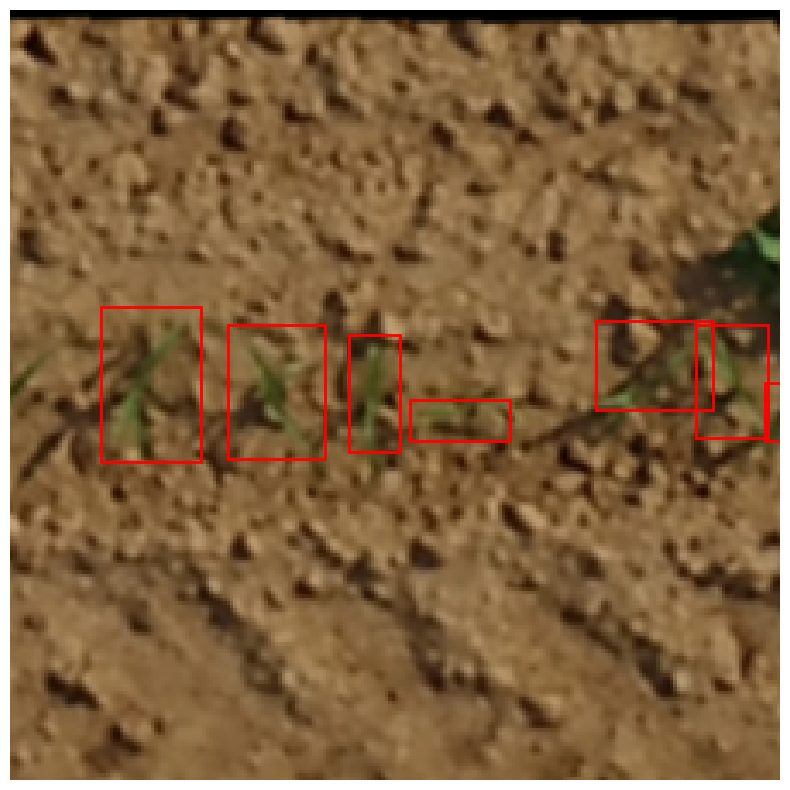
\includegraphics[width=5.5cm]{Plots/DavidEtAl.png}}
  \hfill
  \subfloat[\centering LiuEtAl.2022]{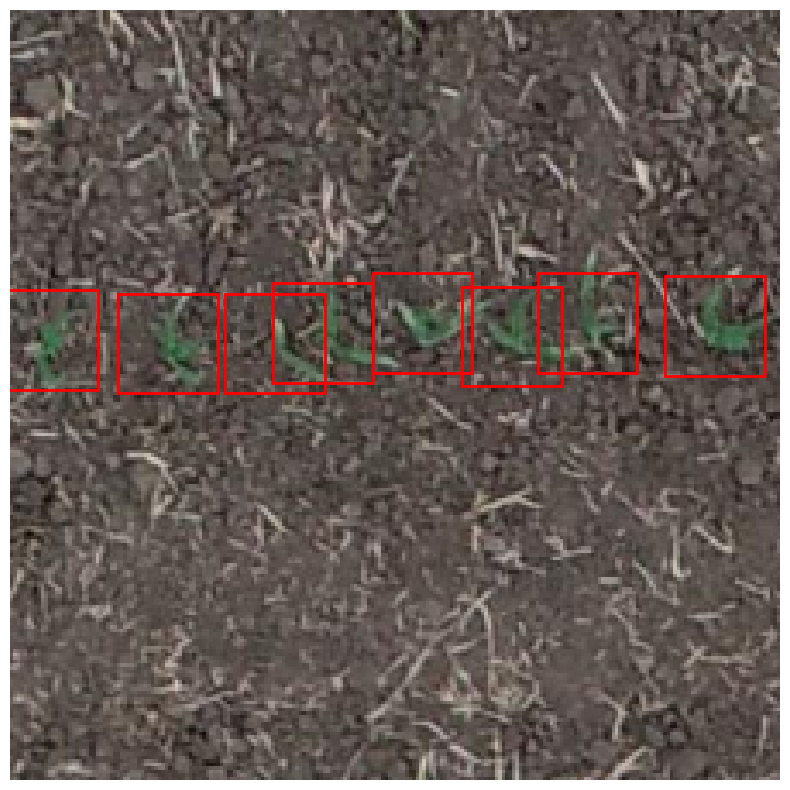
\includegraphics[width=5.5cm]{Plots/LiuEtAl.png}}
  \hfill
  \subfloat[\centering Internet Maize stage V3]{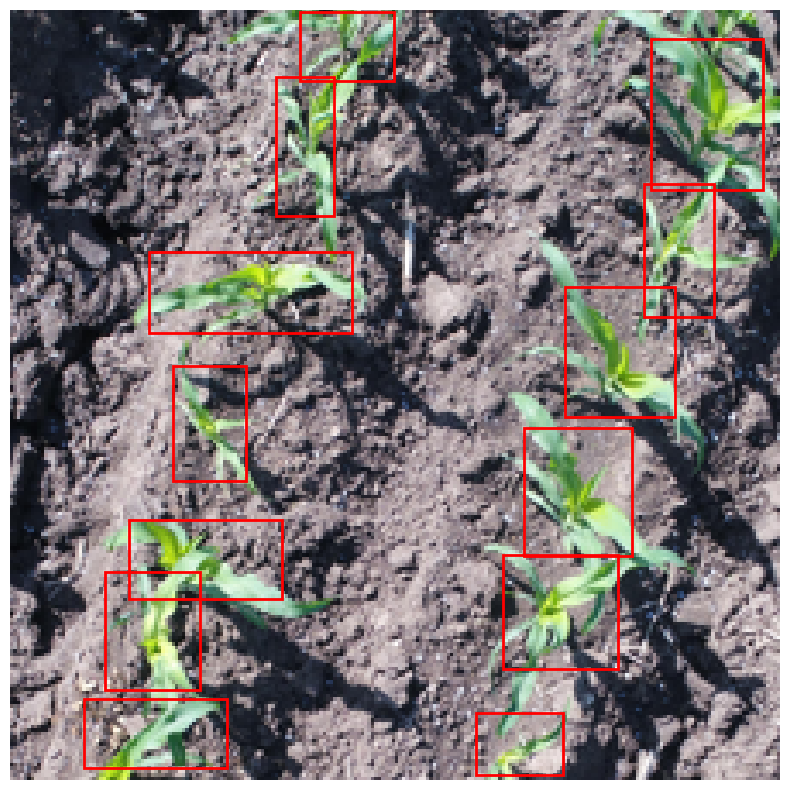
\includegraphics[width=5.5cm]{Plots/maize_seedling.png}}
  \hfill
  \subfloat[\centering Internet Maize stage V5]{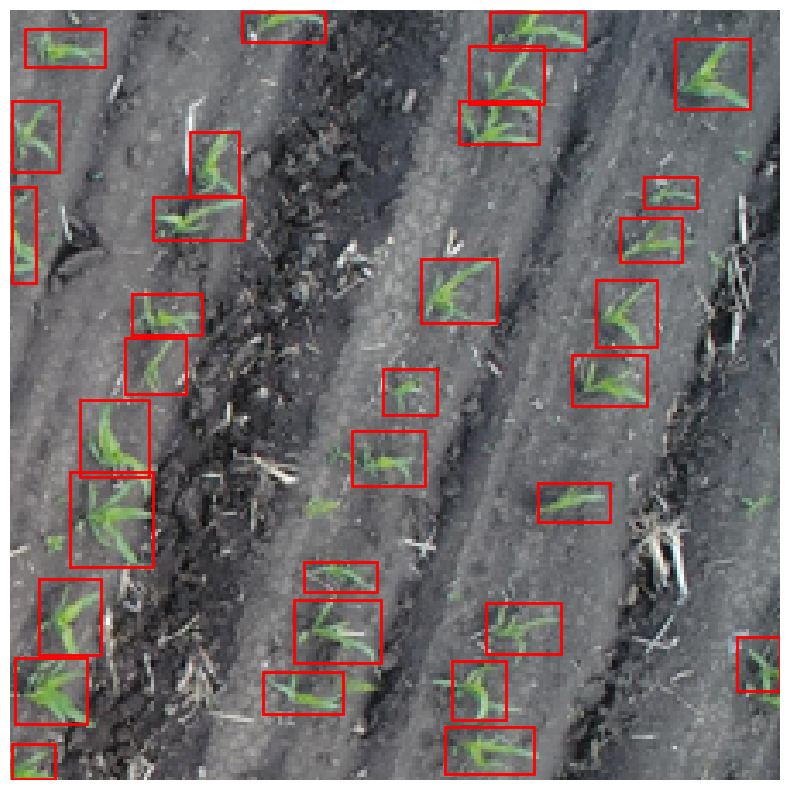
\includegraphics[width=5.5cm]{Plots/maize_seedling_detection.png}}
  
  \vspace{0.5cm}
  % Second row (3 larger images)
  \subfloat[\centering ID\_1]{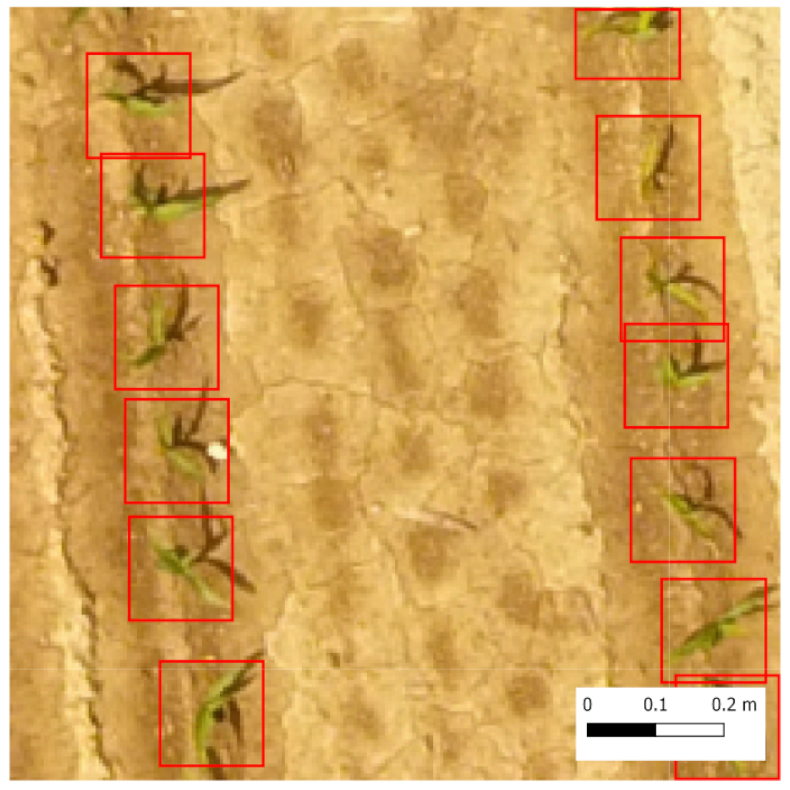
\includegraphics[width=7.5cm]{Plots/ID_1.png}}
  \hfill
  \subfloat[\centering ID\_2]{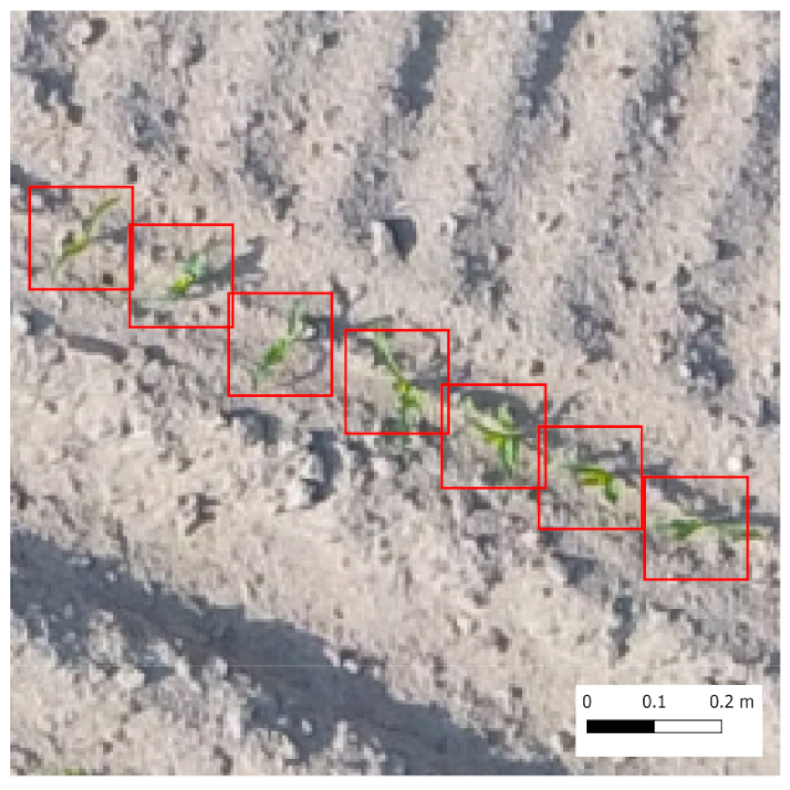
\includegraphics[width=7.5cm]{Plots/ID_2.png}}
  \hfill
  \subfloat[\centering ID\_3]{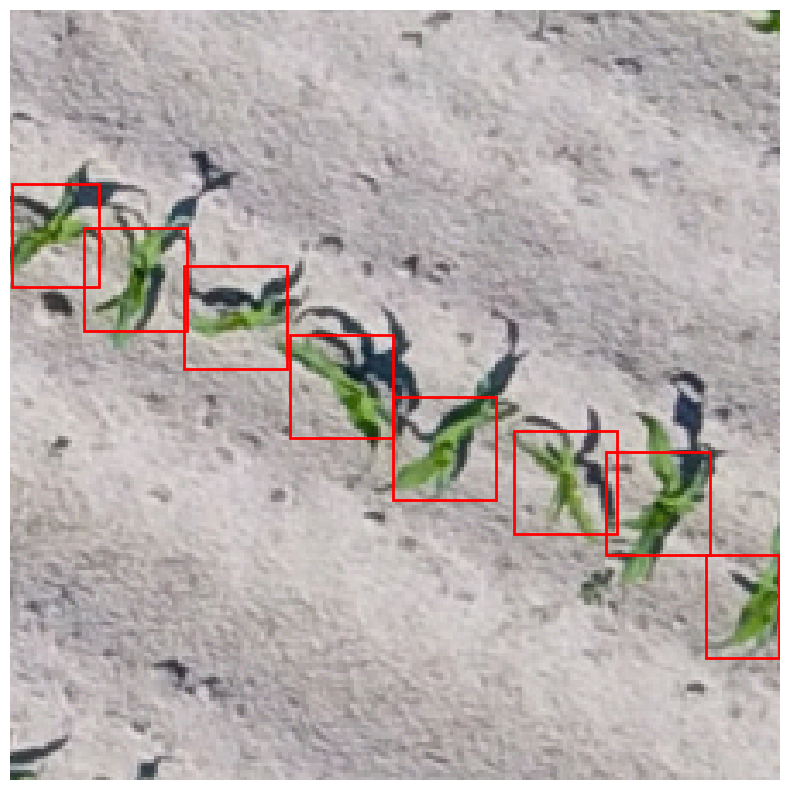
\includegraphics[width=7.5cm]{Plots/ID_3.png}}
  
  \caption{Sample images from each dataset used in the study. The top row shows out-of-distribution datasets: 
  \textbf{(a)} DavidEtAl.2021, \textbf{(b)} LiuEtAl.2022, \textbf{(c)} Internet Maize stage V3, and 
  \textbf{(d)} Internet Maize stage V5. The bottom row shows in-domain datasets: 
  \textbf{(e)} ID\_1, \textbf{(f)} ID\_2, and \textbf{(g)} ID\_3.}
  \label{fig:datasets}  
  \end{adjustwidth}
\end{figure}
\end{landscape}
\clearpage
}


To make the two kind of dataset comparables we chose to rescale the images to a scale of 0.005 m/pixel
where the scale was known (scientific OOD and ID datasets), obtaining orthomosaics of different sizes.
All the orthomosaics were then cropped to 224*224 pixels tiles.
This tile size was selected because at 5 mm/pixel resolution it covers 1.12×1.12 meters of field area.
Given that typical grain maize inter-row distance is 0.75 meters, this size enables capturing 
approximately two rows per tile, which is optimal for row pattern identification in the HC algorithm 
and provides sufficient context for object detection models.
This particular image size was also chosen as a standard from AlexNet \cite{krizhevskyImageNetClassificationDeep2012}
as it should be compatible with most of the object detection architectures.
The annotations were rescaled and cropped where needed.
Figure \ref{fig:datasets} shows a sample for each dataset.
Each ID dataset has 20 tiles to be used as testing dataset, while other 
150 tiles are used as training dataset.

\subsection{Handcrafted object detector}

Like other works \cite{davidPlantDetectionCounting2021,garcia-martinezDigitalCountCorn2020,liuEstimatingMaizeSeedling2022} 
we wrote an HC algorithm to get annotated tiles from the orthomosaics, 
basing it on agronomical knowledge and color thresholding.
Hue, saturation and value (HSV) color space was used here to threshold the image,
to get green pixels, but other color spaces can be used.
For the execution of this algorithm, the following graphical and agronomical 
parameters must be set: color minimum and maximum thresholds (color threshold), the minimum and maximum 
leaf area for plant (leaf area range), the minimum distance between plants on rows (intra-row distance),
and the distance between rows (inter-rows distance). 
The algorithm is expected to works: on orthomosaics of maize seedlings at the V3-V5 growth stage,
with low weeds infestation, with rows having roughly the same angle with meridian and distance between them.

The algorithm is divided in two sequential parts that form a detection-verification pipeline. The first part,
named HC1 \cref{alg:H1}, performs initial plant detection by thresholding pixels within the specified color range, 
identifying connected regions, and filtering them based on expected leaf area. HC1 outputs region polygons
representing potential plants, but typically includes many false positives due to its simple color-based approach.
To address this limitation, we implemented a second process named HC2 (\cref{alg:H2_part1} and \cref{alg:H2_part2}) that applies agronomical 
knowledge of field structure. HC2 filters the HC1 output by verifying that detected plants form proper row 
patterns with expected intra-row and inter-row spacing. It uses RANSAC to identify linear alignments of plants 
and validates that these alignments match expected field geometry (consistent row slope and spacing).
Only tiles where HC2 confirms the expected number and arrangement of plants are retained for the final dataset.
This two-stage approach enables automated extraction of high-confidence annotations from the orthomosaics.

\begingroup
\small
\begin{algorithm}
    \caption{H1}
    \label{alg:H1}
    \begin{algorithmic}[1]
    \Require $tiles$ \Comment{Orthomosaic tiles}
    \Require $col\_range$ \Comment{Color space thresholds}
    \Require $leaf\_area\_range$ \Comment{Leaf area range in pixels}
    \Ensure $plants$ \Comment{List of polygons}
    
    \Function{connected\_components}{$binary\_image$} \cite{wuOptimizingConnectedComponent2005} 
        \State \Return $regions$
    \EndFunction
    
    \For{$tile$ in $tiles$}
      \State $mask \gets \{p \in tile \mid color(p) \in col\_range\}$
      \State $regions \gets connected\_components(mask)$
      \State $plants \gets \{region \mid region \in regions \land region.area \in leaf\_area\_range\}$
    \EndFor
    \State \Return $plants$
  \end{algorithmic}
  \end{algorithm}
  
    
  \begin{algorithm}
  \caption{H2: Part I - Row Detection}
  \label{alg:H2_part1}
  \begin{algorithmic}[1]
  \Require $observations$ \Comment{(List of centroids, RanSaC models)}
  \Require $intra-row\_dist$ \Comment{Minimum distance between plants}
  \Require $inter-row\_dist$ \Comment{Minimum distance between rows}
  \Require $mean\_slope$ \Comment{Mean slope of the rows in respect meridian}
  \Ensure $objects$ \Comment{List of centroids or polygons}
  \Function{region\_centroids}{$regions$} \Comment{Get the centroids of the regions}
    \State \Return $centroids$
  \EndFunction
  \Function{agglomerate\_regions}{$regions, min\_dist$} \Comment{Agglomerate regions}
    \State $centroids \gets \{region.centroid \mid region \in regions\}$
    \State $clusters \gets \text{HierarchicalClustering}(centroids, threshold=min\_dist, metric=\text{euclidean})$
    \State $clust\_cen \gets \{\text{mean}(centroids_i) \mid \text{for each cluster } i \in clusters\}$
    \State \Return $clust\_cen$
  \EndFunction
  \Function{extract\_ransac\_line}{$points,  min\_dist$} \cite{fischlerRandomSampleConsensus1987}
    \State \Return $best\_inliers, best\_model$
  \EndFunction
  \Function{process\_tiles}{$intra-row\_dist$}
    \State $observations \gets \{\}$
    \State $plants \gets \Call{HC1}{tiles}$
    \For{$tile$ in $tiles$}
      \State $regions \gets plants[tile]$
      \State $centroids \gets \Call{region\_centroids}{regions}$
      \State $clust\_cen \gets \Call{agglomerate\_regions}{regions, intra-row\_dist}$
      \State $inlier\_points, model \gets \Call{extract\_ransac\_line}{clust\_cen, intra-row\_dist}$
      \State $line\_length \gets \Call{get\_line\_length}{model}$
      \State $expected\_number\_of\_plants \gets \frac{line\_length}{intra\_row\_dist}$
      \If {$inlier\_points \equiv expected\_number\_of\_plants}$
        \State $observations[tile] \gets (clust\_cen,inlier\_points,model)$
      \EndIf
    \EndFor
    \State \Return $observations$
  \EndFunction
  \end{algorithmic}
  \end{algorithm}
  
  \begin{algorithm}
  \caption{H2: Part II - Row Verification}
  \label{alg:H2_part2}
  \begin{algorithmic}[1]
  \Function{Filter\_observations\_by\_slope}{$observations$}
    \State $filtered\_observations \gets \{\}$
    \For{$tile \in observations$}
      \State $slope \gets observations[tile][\text{'model'}]$
      \If{$model.slope \approx mean\_slope$}
        \State $filtered\_observations[tile] \gets observations[tile]$
      \EndIf
    \EndFor
    \State \Return $filtered\_observations$
  \EndFunction
  \Function{process\_observations}{$observations,inter-row\_dist,intra-row\_dist$}
    \State $objects \gets \{\}$
    \For{$tile \in observations$}
      \State $tile\_centers \gets observations[tile][\text{'clust\_cen'}]$
      \State $first\_row\_centers \gets observations[tile][\text{'inlier\_points'}]$
      \State $first\_row\_model \gets observations[tile][\text{'model'}]$
      \State $centers \gets \{p \mid p \in tile\_centers \land p \notin first\_row\_centers\}$
      \State $second\_row\_centers, second\_row\_model \gets \Call{extract\_ransac\_line}{centers, intra-row\_dist}$
      \State $line\_length \gets \Call{get\_line\_length}{second\_row\_model}$
      \State $expected\_number\_of\_plants \gets \frac{line\_length}{intra\_row\_dist}$
      \If {$second\_row\_model.slope \approx first\_row\_model.slope$}
        \If {$abs(second\_row\_model.intercept - first\_row\_model.intercept) \approx inter-row\_dist$}
          \If {$second\_row\_centers \equiv expected\_number\_of\_plants$}
            \State $objects[tile] \gets (first\_row\_centers, second\_row\_centers)$
          \EndIf
        \EndIf
      \EndIf
    \EndFor
    \State \Return $objects$
  \EndFunction
  \Function{main}{}
    \State $observations \gets \Call{process\_tiles}{intra-row\_dist}$
    \State $MEAN\_SLOPE \gets \Call{mean}{observations[\text{'model'}]}$
    \State $observations \gets \Call{Filter\_observations\_by\_slope}{observations,MEAN\_SLOPE}$
    \State $objects \gets \Call{process\_observations}{observations,inter-row\_dist}$
    \State \Return $objects$
  \EndFunction
  \end{algorithmic}
  \end{algorithm}
\endgroup

\subsection{Deep Learning object detectors}

We chose them for the considerations made in Introduction section~\ref{subsec:object_detection_approaches}.
We used here the Ultralytics implementation of these models because the implementation is open-source \cite{jocherGitHubUltralyticsYOLO2023},
and it makes it possible to tune parameters size coherently across all tested architectures.

All model training and inference was performed on a workstation equipped with an Intel(R) Xeon(R) 
CPU E5-2670 v3 @ 2.30GHz, 64.0 GB RAM, and an NVIDIA RTX A5000 GPU with 24GB VRAM. 
The computational constraints influenced certain experimental design choices, such as 
batch size and precision settings.

For all the many-shots models we used the same hyperparameters and augmentations as the
library default, with the following exceptions:

\begin{itemize}
  \item batch size: 16 (increased from default 8 to maximize GPU utilization while maintaining stable gradients)
  \item maximum training epochs: 200 (extended from default 100 to ensure convergence with small datasets)
  \item maximum training epochs without improvement: 15 (increased from default 10 for early stopping to allow longer plateau exploration)
  \item precision: mixed (to balance training speed and numerical accuracy)
\end{itemize}

The default augmentations from the Ultralytics library include random scaling (±10\%), 
random translation (±10\%), random horizontal flip (probability 0.5), 
HSV color space augmentation (hue ±0.015, saturation ±0.7, value ±0.4), 
and mosaic augmentation. These augmentations were selected to reflect potential 
variations in field conditions without introducing unrealistic distortions.

The training dataset was composed of the OOD or ID training dataset tiles.
For the dataset size testing, all the annotations were used, while for the dataset quality testing
a percentage of the annotations per image was selected and used.

To test the few-shot approach we trained CD-ViTO with multiple model sizes.
The size of this model is determined by the backbone used, which can be ViT-S, ViT-B, or ViT-L \cite{oquabDINOv2LearningRobust2024}. 
We used the implementation of CD-ViTO provided by the authors \cite{fuCrossDomainFewShotObject2024}.
In the context of this study a 'shot' correspond to an image with a single annotated plant. 
We used 1, 5, 10, 30, and 50 shots to train the model.
The shots were randomly selected from the ID manually labeled dataset, then a 
random annotation was selected from the same image to be used as prototype.
All the combinations of shots and ViT backbone were tested on the ID test dataset tiles.

For testing the zero-shot approach we used OWLv2.
We took this architecture as zero-shot object detector example as it is the most stable 
state-of-the-art model for this task \cite{mindererScalingOpenVocabularyObject2023,liuGroundingDINOMarrying2025}.
For test OWLv2 we used the implementation of the transformer library \cite{wolfTransformersStateoftheArtNatural2020}
with the parameters published by the authors.
We tested the encoder sizes ViT-B/16, ViT-L/14 with the following three pre-training 
strategies:

\begin{itemize}
    \item \textbf{Base models}: Trained using self-supervised learning with the OWL-ST method, which generates pseudo-box annotations from web-scale image-text datasets
    \item \textbf{Fine-tuned models}: Further trained on human-annotated object detection datasets
    \item \textbf{Ensemble models}: Combining multiple weight-trained versions to balance open-vocabulary generalization and task-specific performance
\end{itemize}

For all the OWLv2 variants, we tested multiple text prompts to describe maize seedlings, 
ranging from simple terms ("maize", "seedling") to more descriptive phrases 
("aerial view of maize seedlings", "corn seedlings in rows"). The complete list of 
eleven prompts is the following: 
\begin{itemize}
    \item "maize"
    \item "seedling"
    \item "plant"
    \item "aerial view of maize seedlings"
    \item "corn seedlings in rows"
    \item "young maize plants from above"
    \item "crop rows with corn seedlings"
    \item "maize seedlings with regular spacing"
    \item "top-down view of corn plants"
    \item "agricultural field with maize seedlings"
    \item "orthomosaic of corn plants in rows"
\end{itemize}
All the combinations (here named model 
settings) of encoder size, pre-training strategy, and text prompt were tested on the 
ID test dataset tiles.

\cref{tab:architectures} shows the architectures used in the study 
with the parameter size specifics.

\begin{table}[H]
  \caption{Summary of Tested Architectures and Model Sizes\textsuperscript{1}}
  \label{tab:architectures}
  \centering
  \begin{tabularx}{\textwidth}{lXXXXXX}
  \toprule
  \textbf{Architecture} &\textbf{Shots} & \textbf{n\textsuperscript{2}} & \textbf{s\textsuperscript{2} or S} & \textbf{m\textsuperscript{2} or B} & \textbf{l\textsuperscript{2} or L} & \textbf{x\textsuperscript{2}} \\
  \midrule
  YOLOv5 & many & 1.9 & 7.2 & 21.2 & 46.5 & 86.7 \\
  YOLOv8 & many & 3.2 & 11.2 & 25.9 & 43.7 & 68.2 \\
  YOLO11 & many & 4.0 & 12.5 & 28.0 & 50.0 & 75.0 \\
  RT-DETR & many & - & - & - & 60.0 & 80.0 \\
  CD-VITO & few & - & 22.0\textsuperscript{3} & 86.0\textsuperscript{4} & 307.0\textsuperscript{5} & - \\
  OWLv2 & zero & - & - & 86.0\textsuperscript{4} & 307.0\textsuperscript{5} & - \\
  \bottomrule
  \end{tabularx}
  \footnotesize{\textsuperscript{1} Values represent millions of parameters\\
  \textsuperscript{2} Model size variants stand for nano (n), small (s), medium (m), large (l), and extra-large (x)\\
  \textsuperscript{3} ViT-S (Small) backbone\\
  \textsuperscript{4} ViT-B (Base) backbone\\
  \textsuperscript{5} ViT-L (Large) backbone}
\end{table}

\subsection{Minimum dataset size and quality modelling}
In order to investigate the minimum size and quality of the dataset required to train 
a robust object detection model for maize seedlings counting, we conducted a series of experiments
where the above mentioned DL models were recursivelly fitted with increasing dataset size and quality.
For many-shots models we consider a training 
dataset split of 10\% validation and 90\% training, while for few-shots the number of shots
determined the amount of training samples. Zero-shots relied only on descriptions 
in natural language of the objects to be detected.
For what concerns only the dataset size evaluation, for many-shots models we considered
sizes from 10 to 150 images in 15 steps of 10 images, while for few-shots models we considered
1, 5, 10, 30, and 50 shots.
For what concerns the dataset quality, we evaluated the annotation quality by reducing
the number of annotations per image from 100\% to 10\% in 10 steps of 10\% while
keeping the dataset size constant.

For all the models we evaluated the relationship between dataset size or quality and model performance
using $R^2$ and $mAP$, respectively for plant countig and plant detection. Wheter 
$R^2$ provided values below -1 we also considered $RMSE$ as metric for counting.
MAPE was considered for few-shots and zero-shots models only to evaluate the 
quality of the annotations produced by the prediction of these models.
We list here the metrics formulas for clarity:

\begin{align}
R^2 &= 1 - \frac{\sum_{i=1}^{n} (y_i - \hat{y}_i)^2}{\sum_{i=1}^{n} (y_i - \bar{y})^2}
\end{align}

where $y_i$ is the ground truth count for the $i$-th image, $\hat{y}_i$ is the 
predicted count, and $\bar{y}$ is the mean of all ground truth counts. $R^2$ ranges 
from $-\infty$ to 1, with 1 indicating perfect prediction, 0 indicating that the 
model predictions are no better than simply predicting the mean, and negative 
values indicating that the model performs worse than predicting the mean.

\begin{align}
\text{$RMSE$} &= \sqrt{\frac{1}{n}\sum_{i=1}^{n} (y_i - \hat{y}_i)^2}
\end{align}

where $RMSE$ measures the average magnitude of prediction errors in the original 
units (number of plants).

\begin{align}
\text{MAPE} &= \frac{100\%}{n}\sum_{i=1}^{n} \left| \frac{y_i - \hat{y}_i}{y_i} \right|
\end{align}

where MAPE measures the percentage error relative to the actual values, providing a scale-independent 
measure of accuracy. It is expressed as a percentage, with lower values indicating lower
percentage of false positive or false negative.
Thus it was reported as an index of the quality of the annotations.
Note that MAPE is only calculated for cases where $y_i \neq 0$ to avoid division by zero.
It is particular useful for counting as testing tiles never have zero plants.

For object detection performance, we used the standard COCO evaluation metric:

\begin{align}
\text{$mAP$} &= \frac{1}{|IoU|}\sum_{t \in IoU}\text{AP}_t
\end{align}

where $mAP$ (mean Average Precision) is calculated at a single IoU (Intersection over Union) 
threshold of 0.5.
AP at the IoU threshold is the area under the precision-recall curve for detections 
that meet that IoU threshold criterion.

To test the predictability minimum dataset size and quality required to train a robust
(achieving benchmark) object detector for maize seedlings counting through empirical 
models, we test the logarithmic, arctan and algebraic root functions to fit the 
dataset size or quality versus performance relationships as suggested by previous
studies \cite{mahmoodHowMuchMore2022}. 
For clarity we list here the functions tested:


\begin{align}
\text{Logarithmic: } f(x) &= a \ln(x) + b
\end{align}

\begin{align}
\text{Arctan: } f(x) &= a \arctan(bx) + c
\end{align}

\begin{align}
\text{Algebraic Root: } f(x) &= a x^{1/b} + c
\end{align}

For the model fits to dataset size versus performance relationships, we evaluated 
multiple fitting functions and selected the one with the highest goodness-of-fit:

\begin{align}
\text{$GoF$} &= R^2_{\text{fit}} = 1 - \frac{\sum_{i=1}^{n} (y_i - f(x_i))^2}{\sum_{i=1}^{n} (y_i - \bar{y})^2}
\end{align}

where $y_i$ is the observed metric (either $R^2$ or $mAP$), $f(x_i)$ is the 
fitted value at dataset size $x_i$, and $\bar{y}$ is the mean of the observed 
metrics.

All the trained models were tested on the testing dataset tiles with the SAHI method \cite{akyonSlicingAidedHyper2022}.
The SAHI method slices the testing image into smaller overlapping segments (patches) 
of the same size as the training tiles and then tests the model on each of them. 
The model outputs from each patch are then merged by non-maximum suppression and 
cropped by the original tile extension.
The use of such a method is justified by the fact that the model is trained on tiles and
the testing dataset is composed by tiles, but the real application is on orthomosaics, so
the same object can be present in more than one tile in a cutted (and occluded) way.
The SAHI method overcomes this problem ensuring all the possible objects are evaluated by the
model as a whole. Thus it is expected to give a better performance in respect to the use of the
single tile as input for the model.
The prediction were then thresholded by a list of confidence score thresholds to get the plant count.
All the metrics were computed for different score thresholds for all the models
to evaluate the model performance at different confidence levels.
The values to thresholds bounding boxes score were: 0, 0.05, 0.1, 0.15, 0.2, 0.25, 0.29, 0.4, 0.5, 0.6, 0.7, 0.8, 0.9, 0.95, 0.99.
The highest $R^2$ value whithin the thresholds was considered as the model 
performance for that experiment.
%%%%%%%%%%%%%%%%%%%%%%%%%%%%%%%%%%%%%%%%%%
\section{Results}

\subsection{Handcrafted object detector}

To evaluate the HC object detector as a training dataset extractor from the ID dataset,
we measure the amount of annotated tiles that the HC algorithm can extract from the orthomosaics
and the accuracy it delivers in comparison to handmade annotations.
Table \ref{tab:HC_results} shows the performance of the HC object detector on the ID datasets 
by enumerating metrics and successfully annotated tiles. The metrics were computed
on the testing dataset tiles.

\begin{table}[H]
  \caption{HC Object Detector Performance}
  \label{tab:HC_results}
  \centering
  \begin{tabularx}{\textwidth}{lXXXXXX}
  \toprule
  \textbf{Dataset} & \textbf{$R^2$} & \textbf{$RMSE$} & \textbf{$MAPE$} & \textbf{$mAP$} & \textbf{tiles} & \textbf{dataset \%} \\
  \midrule
  ID\_1 & 0.95 & 0.12 & 9\% & 0.87 & 1184 & 7.8\% \\
  ID\_2 & 0.93 & 0.11 & 12\% & 0.81 & 279 &  4.2\% \\
  ID\_3 & 0.87 & 0.18 & 16\% & 0.73 & 158 & 1.8\% \\
  \bottomrule
  \end{tabularx}
  \end{table}

Overall the HC object detector performed well on the ID datasets, with $R^2$ values
above 0.85 for all the datasets. The $RMSE$ values were below 0.2, while the $mAP$ values
were above 0.7. The MAPE values were below 20\% for all the datasets.
The HC algorithm was able to extract a significant amount of annotated tiles from the orthomosaics,
with a percentage of the dataset ranging from 1.8\% to 7.8\%.
In nominal scale the number of tiles successfully annotated by the HC algorithm was
not constant, but always over 150 tiles, so we took this minimum amount as 
maximum dataset size for the many-shots training.

\subsection{Many-shots object detectors}

\subsubsection{OOD training}

The OOD scientific datasets "DavidEtAl.2021" and "LiuEtAl.2022" were tested singularly 
and in combination in the experiment named "scientific OOD". The OOD internet datasets "internet OOD"
were tested singularly and in combination with the OOD scientific datasets in the experiment named "All OOD".
Each model and OOD dataset combination was tested on the testing dataset tiles of the three ID datasets.

\afterpage{%
\clearpage
\begin{landscape}
\begin{figure}[p]
  \centering
  \begin{adjustwidth}{-0cm}{1cm}
  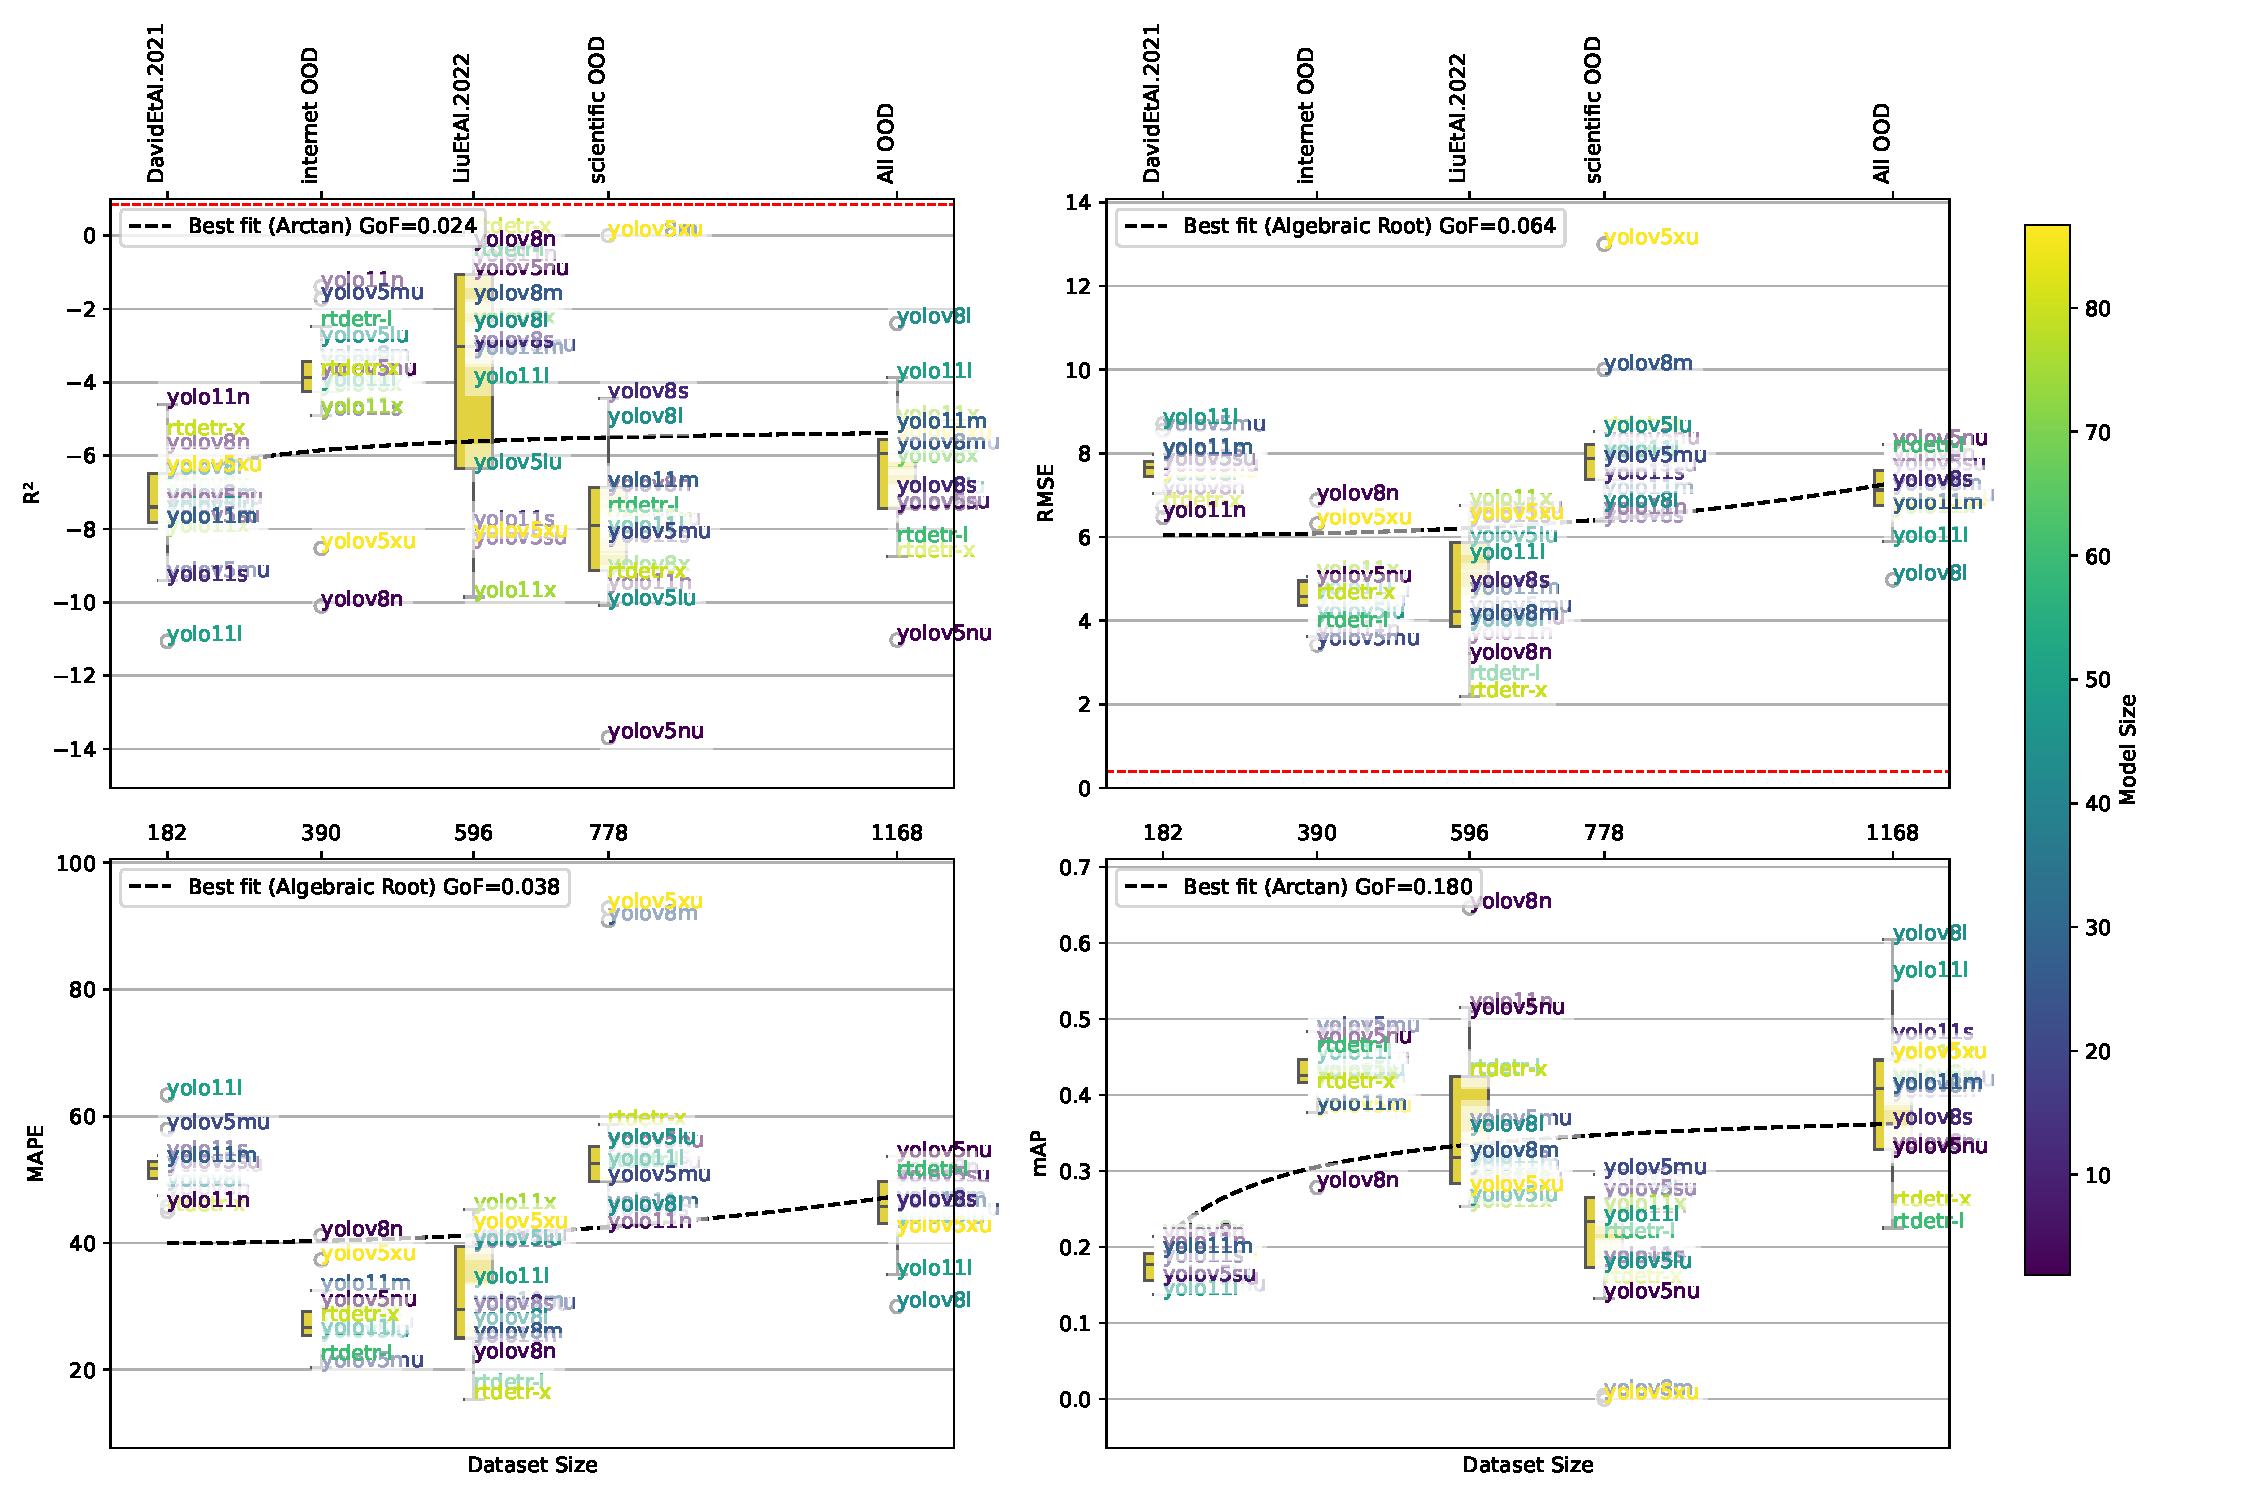
\includegraphics[width=1\linewidth]{Plots/metrics_OOD_datasets.pdf}
  \end{adjustwidth}
  \caption{Performance of the many-shots object detection models 
  trained on 
  the different out-of-distribution (OOD) datasets. Subplots represent: 
  R², $RMSE$, MAPE, and $mAP$ respectively at the right top, left top, left bottom, and right bottom.
  Each subplot contains the boxplots
  positioned at the corresponding dataset size values and indicating the distribution of
  all the models prediction metric values for each dataset.
  Each data point is annotated with the , colored according 
  to the model size. Benchmark thresholds are indicated with red 
  dashed horizontal lines for R² (0.85) and $RMSE$ (0.39). Best fit lines for each metric are 
  plotted using different fitting functions (logarithmic, arctan, and algebraic root), 
  indicated with black dashed lines. $GoF$ values and best model are shown in the
  legend.
  A secondary x-axis at the top of each subplot 
  shows the dataset names corresponding to the dataset sizes.}
  \label{fig:metrics_OOD_datasets}
\end{figure}
\end{landscape}
\clearpage
}

None of the dataset combinations reached the benchmark $R^2$ value of 0.85 with any model.
The coefficients of determinations and the root mean square errors 
for all the OOD experiments are shown in Figure \ref{fig:metrics_OOD_datasets}.
The Goodness-of-fit ($GoF$) values for the $R^2$ values were always low (below 0.2) for all the metrics.
The lowest $MAPE$ value was slightly less than 20\%. For these same models the $mAP$ values
were the highest, with the best model being YOLOv8n with the LiuEtAl.2022 dataset.
No particular model size seems to provide better results with respect to the others,
neither the increasing dataset size seems to drive a model size performance trend.
As no model achieved the benchmark, no study was done on the dataset quality requirements
to achieve such benchmark.

\subsubsection{ID training}

The relationship between ID training dataset size and model performance was evaluated 
for all model architectures and sizes as shown in Figures~\ref{fig:dataset_size_vs_performance_yolov5},
\ref{fig:dataset_size_vs_performance_yolov8},
\ref{fig:dataset_size_vs_performance_yolo11} and
\ref{fig:dataset_size_vs_performance_rtdetr}. 
The dataset quality was tested later, taking the combination of model architecture, model size and
training dataset size that achieved the benchmark and retraining that model while reducing the amount of
annotations for each tile. 
The $R^2$ values of the counting and the $mAP$ values for all models were regressed 
against the dataset size using a logarithmic, root or arctan model. The best fitting
whitin them was selected for each model and metric and the $GoF$ was calculated.
A high $GoF$ value indicates that model performance is highly predictable by dataset size. 
Conversely, a poor $GoF$ could indicate that other variables play a more important 
role in determining model performance, or that the chosen dataset size interval is 
too narrow to achieve a good fit.

% First subfigure (YOLOv5)
\afterpage{%
\clearpage
\begin{landscape}
\begin{figure}[p]
  \centering
  \begin{adjustwidth}{-5cm}{-0cm}  % Increase margins on both sides
  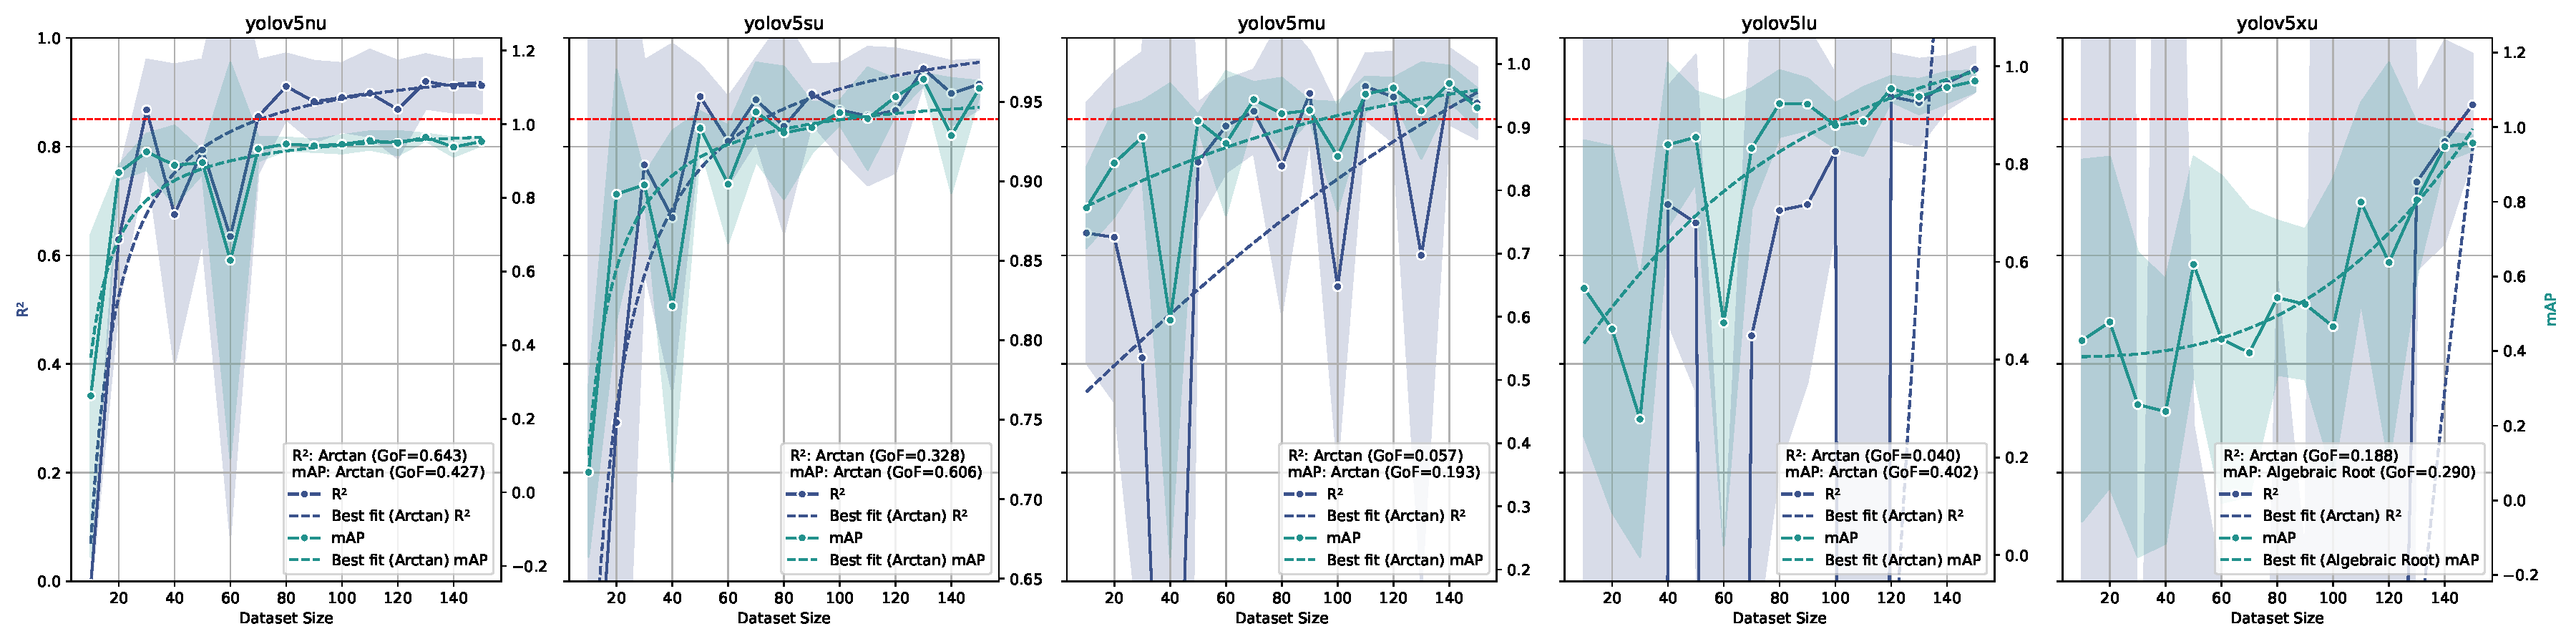
\includegraphics[width=1\linewidth]{Plots/r2_ap_vs_dataset_size_yolov5.pdf}
  \end{adjustwidth}
  \caption[Dataset size vs. model performance (YOLOv5)]{Relationship between dataset size and model performance 
  for YOLOv5 trained and tested on ID datasets. 
  Each subplot represents a different parameters size of the model,
  increasing from the left to the right. The x-axis represents the dataset size, while
  the left and right y-axis represents the $R^2$ and $mAP$ values respectively. 
  The solid lines represent the mean values, while the dashed lines indicate the logarithmic fit.
  The shaded area around the solid lines represents the confidence interval (standard
  deviation) of $R^2$ or $mAP$. The red dashed horizontal line represents the benchmark $R^2$ value of 0.85.
  The legend shows the goodness of fit ($GoF$) for both $R^2$ and $mAP$.}
  \label{fig:dataset_size_vs_performance_yolov5}  
\end{figure}
\end{landscape}
\clearpage
}

% Second subfigure (YOLOv8)
\afterpage{%
\clearpage
\begin{landscape}
\begin{figure}[p]
  \centering
  \begin{adjustwidth}{-5cm}{-0cm}
  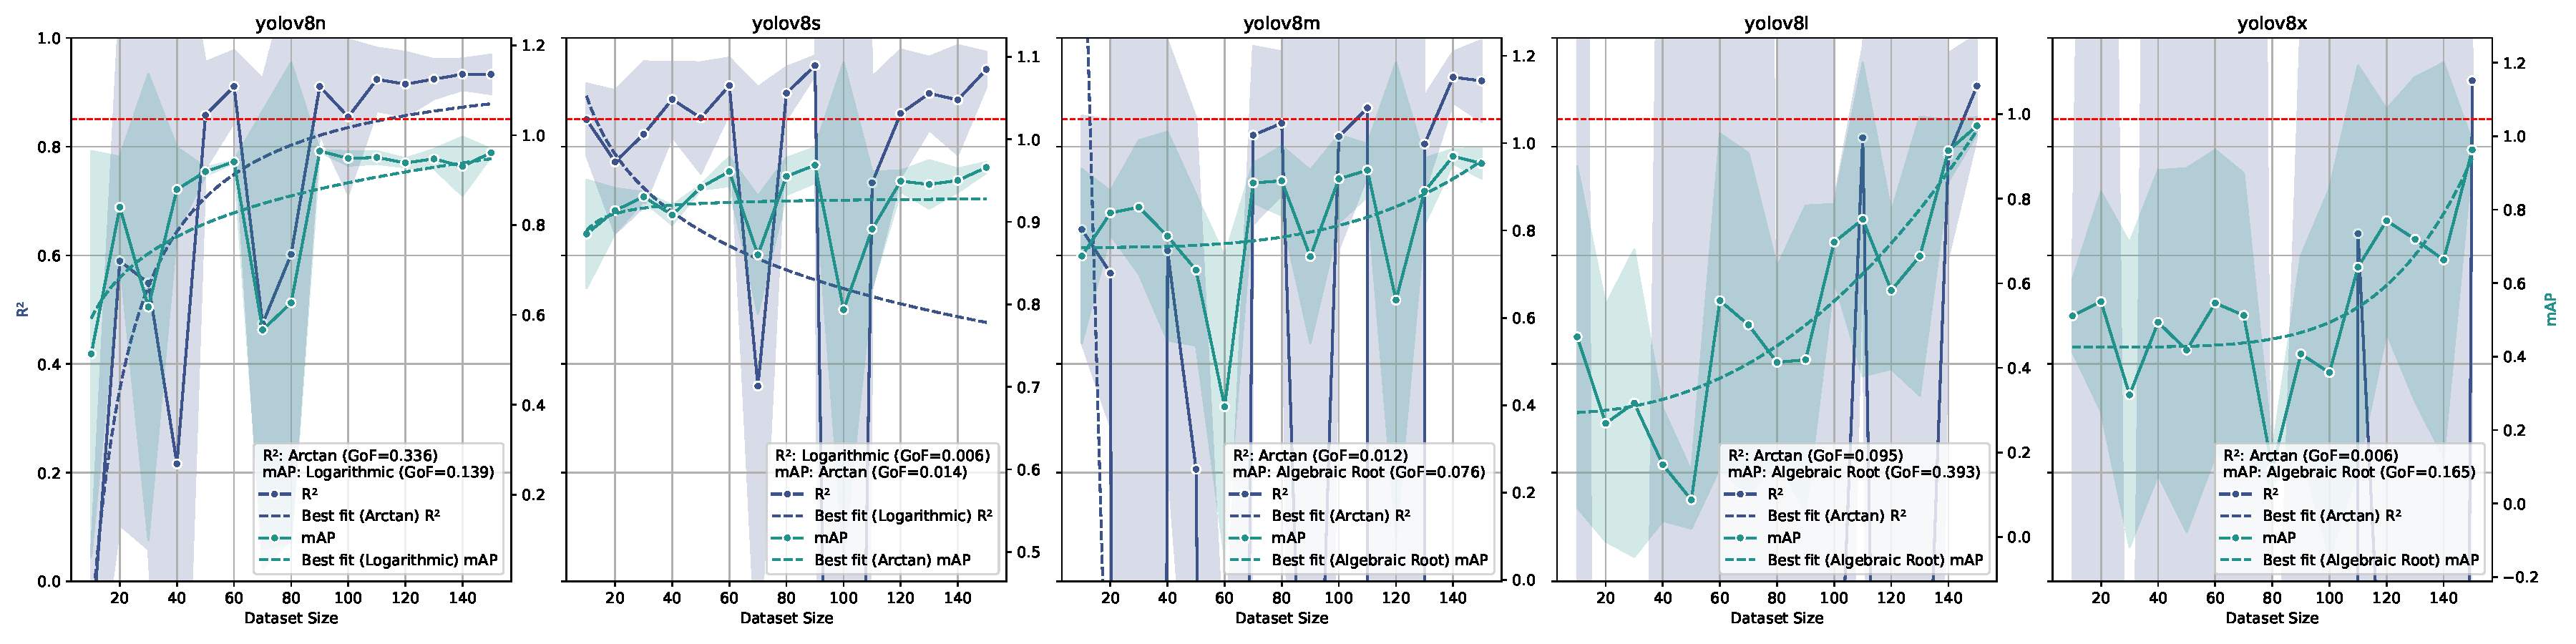
\includegraphics[width=1\linewidth]{Plots/r2_ap_vs_dataset_size_yolov8.pdf}
  \end{adjustwidth}
  \caption[Dataset size vs. model performance (YOLOv8)]{Relationship between dataset size and model performance 
  for YOLOv8 trained and tested on ID datasets. 
  Each subplot represents a different parameters size of the model,
  increasing from the left to the right. The x-axis represents the dataset size, while
  the left and right y-axis represents the $R^2$ and $mAP$ values respectively. 
  The solid lines represent the mean values, while the dashed lines indicate the logarithmic fit.
  The shaded area around the solid lines represents the confidence interval (standard
  deviation) of $R^2$ or $mAP$. The red dashed horizontal line represents the benchmark $R^2$ value of 0.85.
  The legend shows the goodness of fit ($GoF$) for both $R^2$ and $mAP$.}
  \label{fig:dataset_size_vs_performance_yolov8}  
\end{figure}
\end{landscape}
\clearpage
}

% Third subfigure (YOLO11)
\afterpage{%
\clearpage
\begin{landscape}
\begin{figure}[p]
  \centering
  \begin{adjustwidth}{-5cm}{-0cm}
  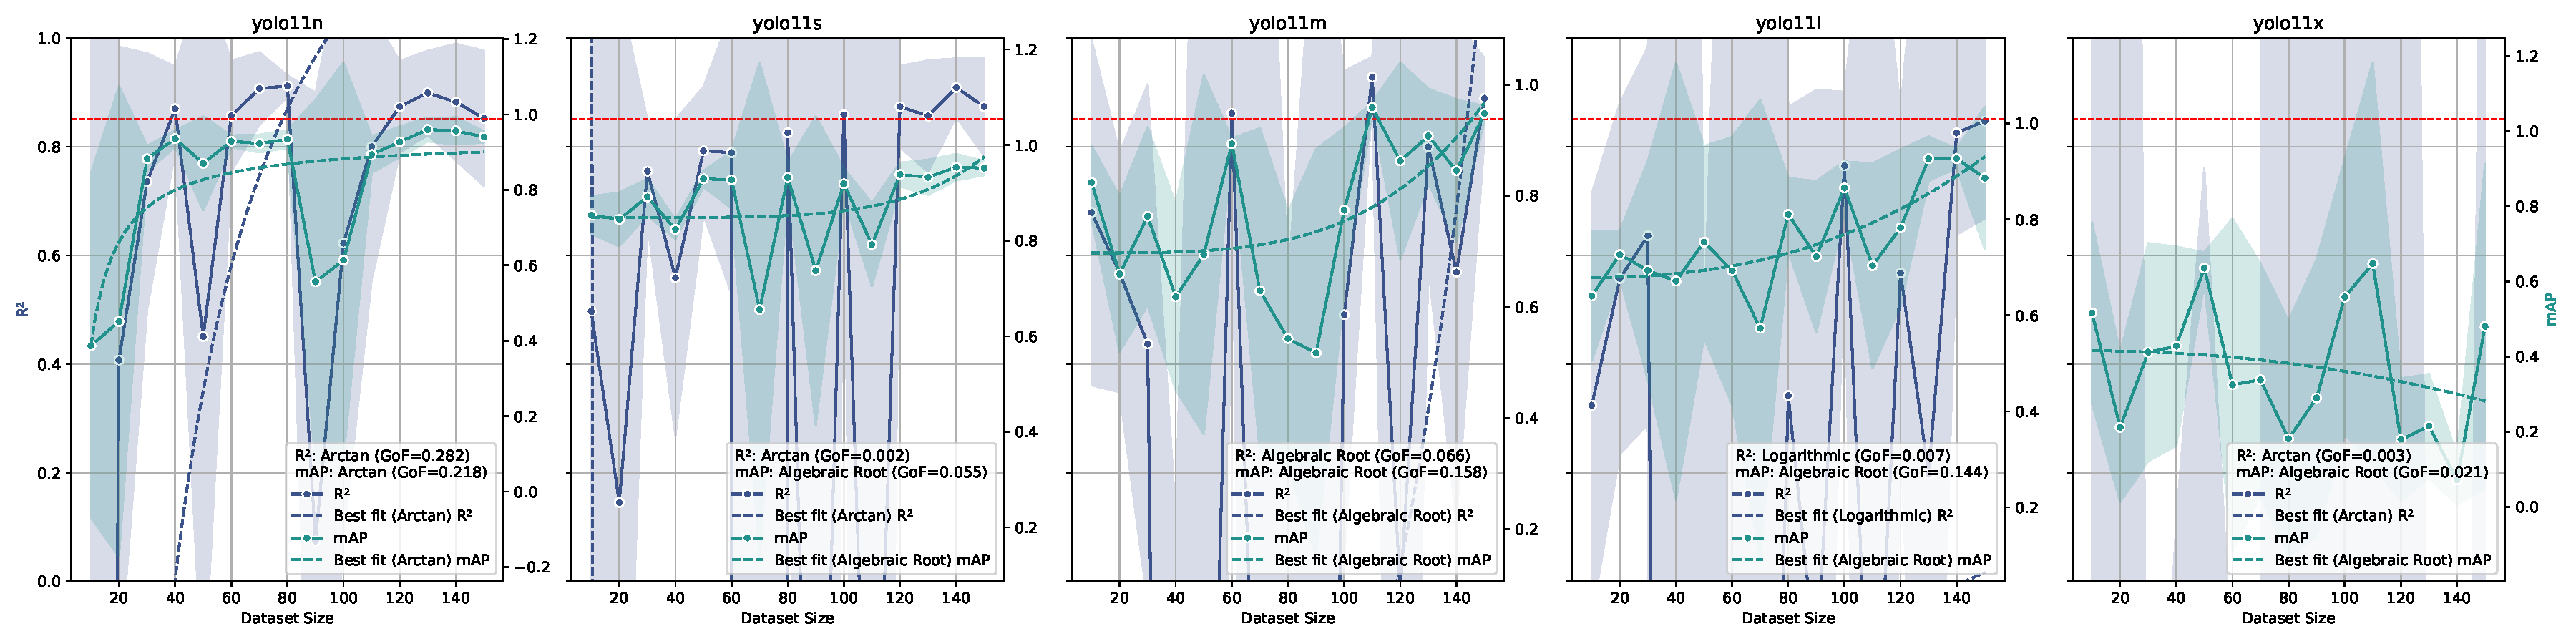
\includegraphics[width=1\linewidth]{Plots/r2_ap_vs_dataset_size_yolo11.pdf}
  \end{adjustwidth}
  \caption[Dataset size vs. model performance (YOLO11)]{Relationship between dataset size and model performance 
  for YOLO11 trained and tested on ID datasets. 
  Each subplot represents a different parameters size of the model,
  increasing from the left to the right. The x-axis represents the dataset size, while
  the left and right y-axis represents the $R^2$ and $mAP$ values respectively. 
  The solid lines represent the mean values, while the dashed lines indicate the logarithmic fit.
  The shaded area around the solid lines represents the confidence interval (standard
  deviation) of $R^2$ or $mAP$. The red dashed horizontal line represents the benchmark $R^2$ value of 0.85.
  The legend shows the goodness of fit ($GoF$) for both $R^2$ and $mAP$.}
  \label{fig:dataset_size_vs_performance_yolo11}  
\end{figure}
\end{landscape}
\clearpage
}

% Fourth subfigure (RT-DETR)
\afterpage{%
\clearpage
\begin{landscape}
\begin{figure}[p]
  \centering
  \begin{adjustwidth}{-5cm}{-0cm}
  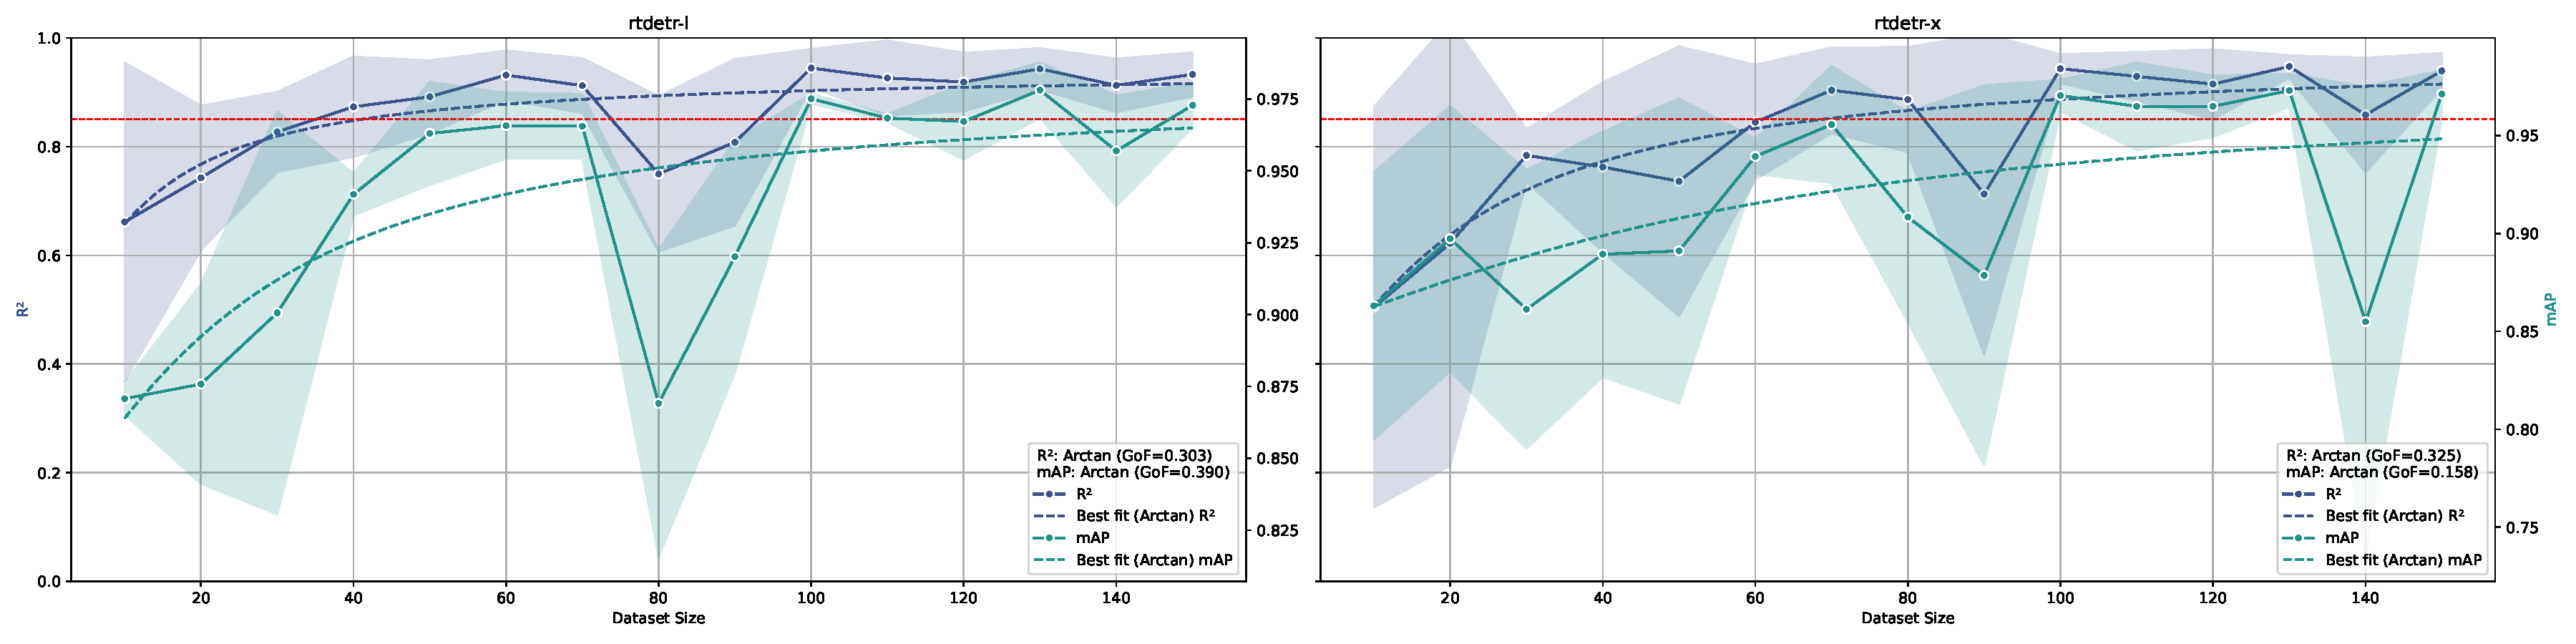
\includegraphics[width=1\linewidth]{Plots/r2_ap_vs_dataset_size_rtdetr.pdf}
  \end{adjustwidth}
  \caption[Dataset size vs. model performance (RT-DETR)]{Relationship between dataset size and model performance 
  for RT-DETR trained and tested on ID datasets. 
  Each subplot represents a different parameters size of the model,
  increasing from the left to the right. The x-axis represents the dataset size, while
  the left and right y-axis represents the $R^2$ and $mAP$ values respectively. 
  The solid lines represent the mean values, while the dashed lines indicate the logarithmic fit.
  The shaded area around the solid lines represents the confidence interval (standard
  deviation) of $R^2$ or $mAP$. The red dashed horizontal line represents the benchmark $R^2$ value of 0.85.
  The legend shows the goodness of fit ($GoF$) for both $R^2$ and $mAP$.}
  \label{fig:dataset_size_vs_performance_rtdetr}  
\end{figure}
\end{landscape}
\clearpage
}

\afterpage{%
\clearpage
\begin{landscape}
\begin{figure}[p]
  \centering
  \begin{adjustwidth}{-5cm}{-0cm}
  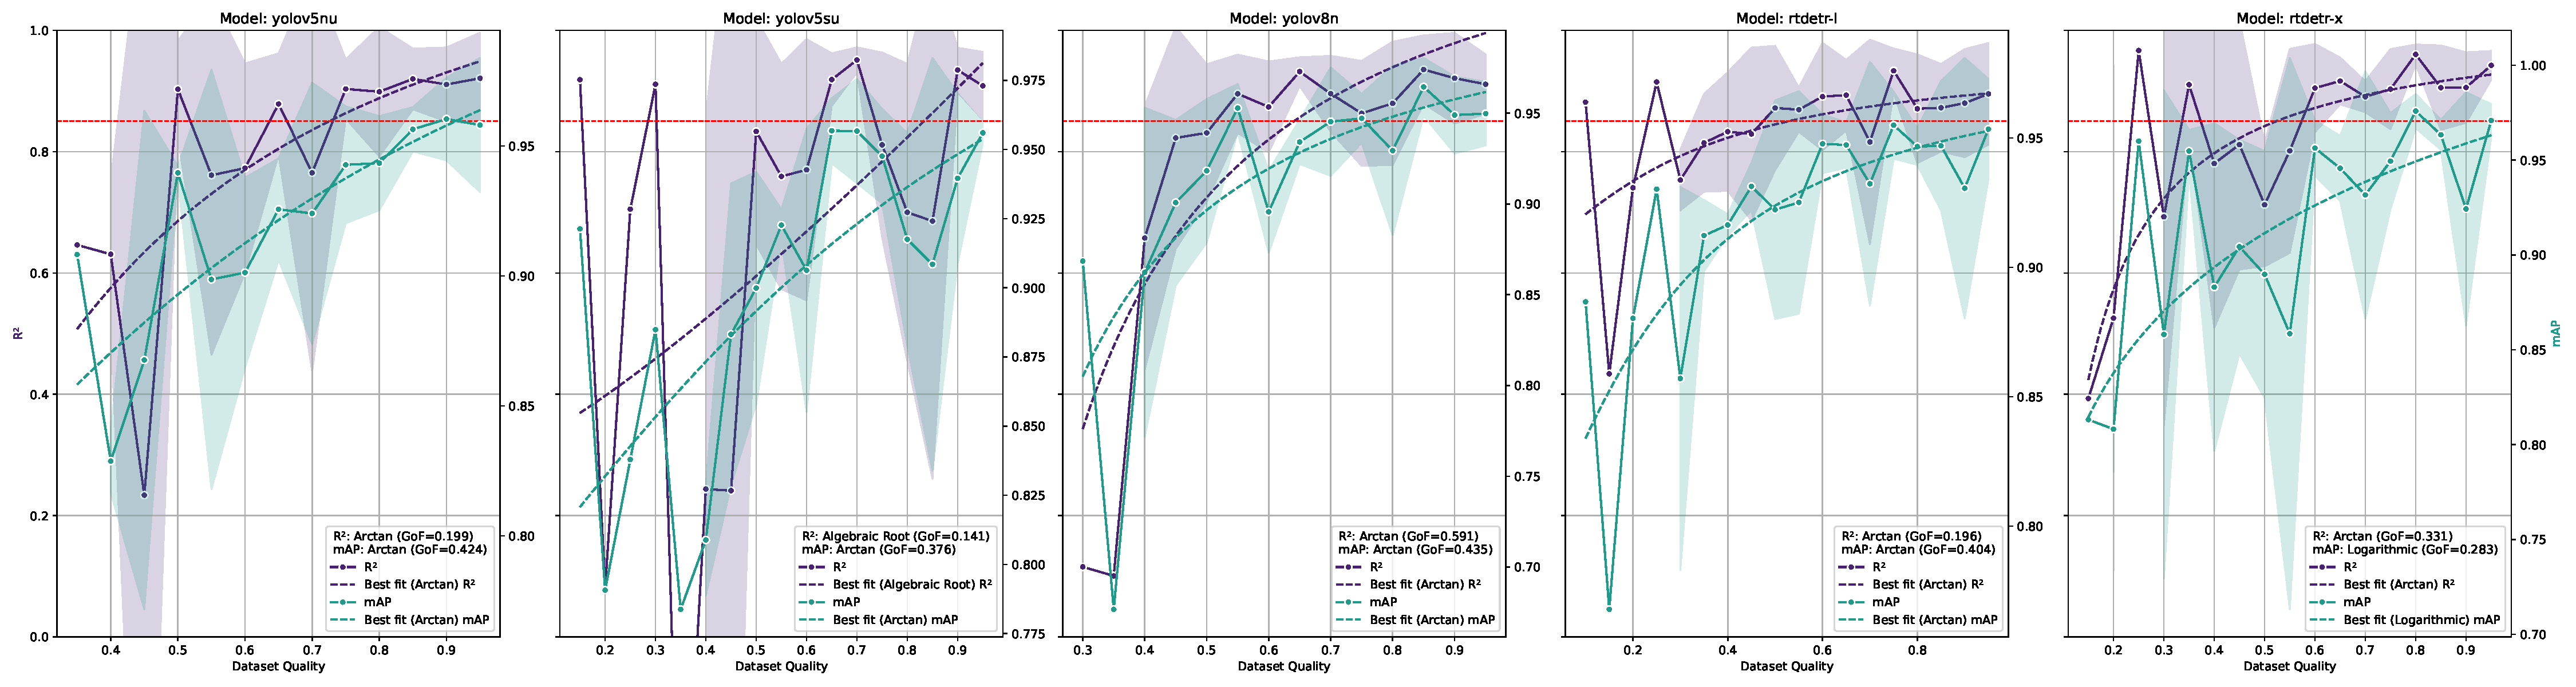
\includegraphics[width=1\linewidth]{Plots/r2_ap_vs_dataset_quality.pdf}
  \end{adjustwidth}
  \caption{Relationship between dataset quality and model performance for all object detection models
  that achieved the benchmark. The x-axis represents the dataset quality, while 
  the left y-axis represents the $R^2$ values.
  The red dashed horizontal line represents the benchmark $R^2$ value of 0.85. The
  legend in the lower right corner of the subplot shows the goodness of fit ($GoF$) for $R^2$.}
  \label{fig:dataset_quality}
\end{figure}
\end{landscape}
\clearpage
}

For the combinations of model-architecture/dataset-size that achieved the benchmark,
the minimum dataset quality required to achieve the benchmark was evaluated as
shown in Figure~\ref{fig:dataset_quality}. The minimum dataset quality was determined by identifying 
the quality percentage where both the empirical model prediction and the entire confidence interval 
of the performance metrics remained above the benchmark threshold.

Within YOLO models, YOLOv5n, YOLOv5s and YOLOv8n achieve the benchmark $R^2$ 
value of 0.85 with 130, 130 and 110 samples, respectively, considering the dataset
sizes where all three model performances were above 0.85 $R^2$ and the logarithmic
model predicted over-benchmark values for that dataset size.
RT-DETR L and RT-DETR X achieve the benchmark $R^2$ value of 0.85 with 60 and 100 samples
respectively, with the same assumptions as for YOLO models.
For these models the $GoF$ was above 0.3, while for the models that did
not reach the benchmark $R^2$ value the $GoF$ was always below this value.
The $mAP$ seems to follow the same trend as the $R^2$ values.
All the models show a clear trend of increasing $R^2$ and $mAP$
values as the dataset size increases, as expected.
It is also clear that increasing number of parameters and model complexity for
mostly CNN-like models (YOLOs) leads to increasing need for dataset size.
For the mostly transformer-like models (RT-DETRs) it is not that clear, also because of
the low amount of model parameter sizes tested.
The confidence interval reduction as a function of the dataset size indicates that 
variability in performance decreases significantly as dataset size increases for 
all models.
Taking into account the dataset quality in the same way as done for the dataset size,
both quality tests and quality models achieved the benchmark with 85\%, 90\%, 85\% and
65\% of the original dataset quality for YOLOv5n, YOLOv5s, YOLOv8n and RT-DETR X, respectively.
RT-DETR L did not achieve the benchmark for any dataset quality reduction tested.

\subsection{Few-shots object detectors}

The few-shots models were evaluated against the established benchmarks ($R^2$ of 0.85 and $RMSE$ of 0.39) 
using the metrics $R^2$ and $RMSE$ because none of the models reached these benchmarks.

\afterpage{%
\clearpage
\begin{landscape}
\begin{figure}[p]
  \centering
  \begin{adjustwidth}{-5cm}{-0cm}
  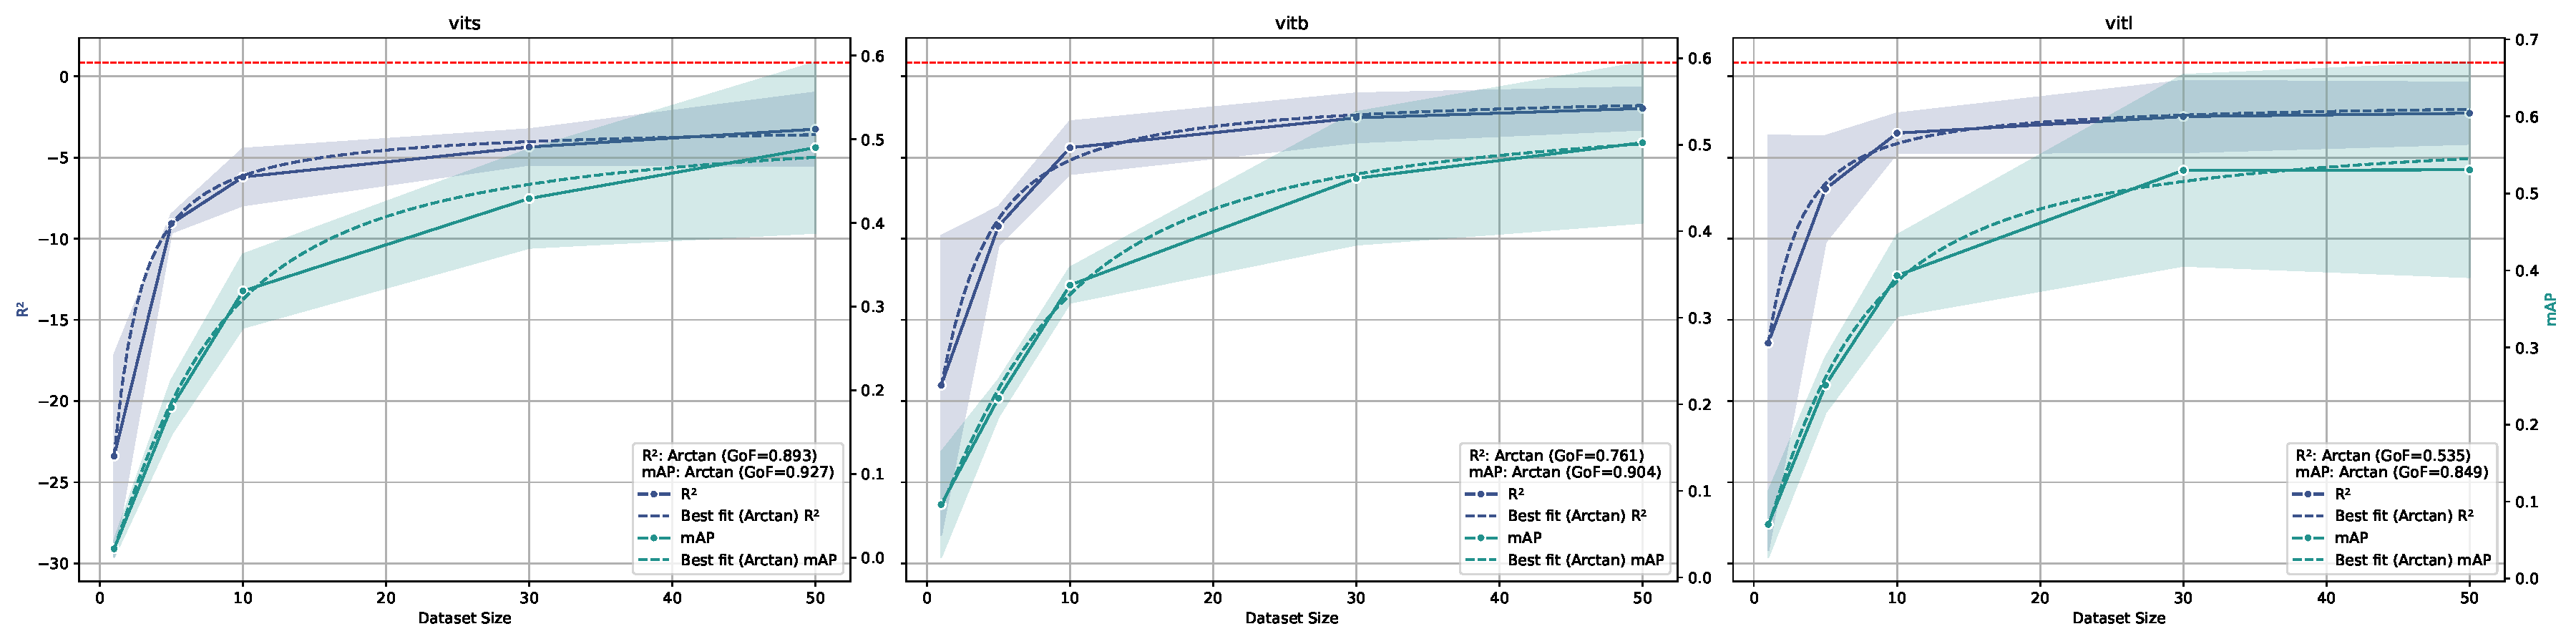
\includegraphics[width=1\linewidth]{Plots/r2_ap_vs_shots_cdvito.pdf}
  \end{adjustwidth}
  \caption{The figure shows the relationship between shots and model performance
  for the CD-ViTO model trained and tested on ID datasets.
  The x-axis represents the number of shots.
  The solid lines represent the mean values, while the dashed lines indicate the shots amount/metric 
  prediction model. The left and right y-axis represents the $R^2$ and $mAP$ values respectively.
  The red dashed horizontal line represents the benchmark $R^2$ value of 0.85. The combined
  legend in the lower right corner of each subplot shows the goodness of fit ($GoF$) for both $R^2$
  and $mAP$.}
  \label{fig:shots_vs_performance1}
\end{figure}
\end{landscape}
\clearpage
}

\afterpage{%
\clearpage
\begin{landscape}
\begin{figure}[p]
  \centering
  \begin{adjustwidth}{-5cm}{-0cm}
  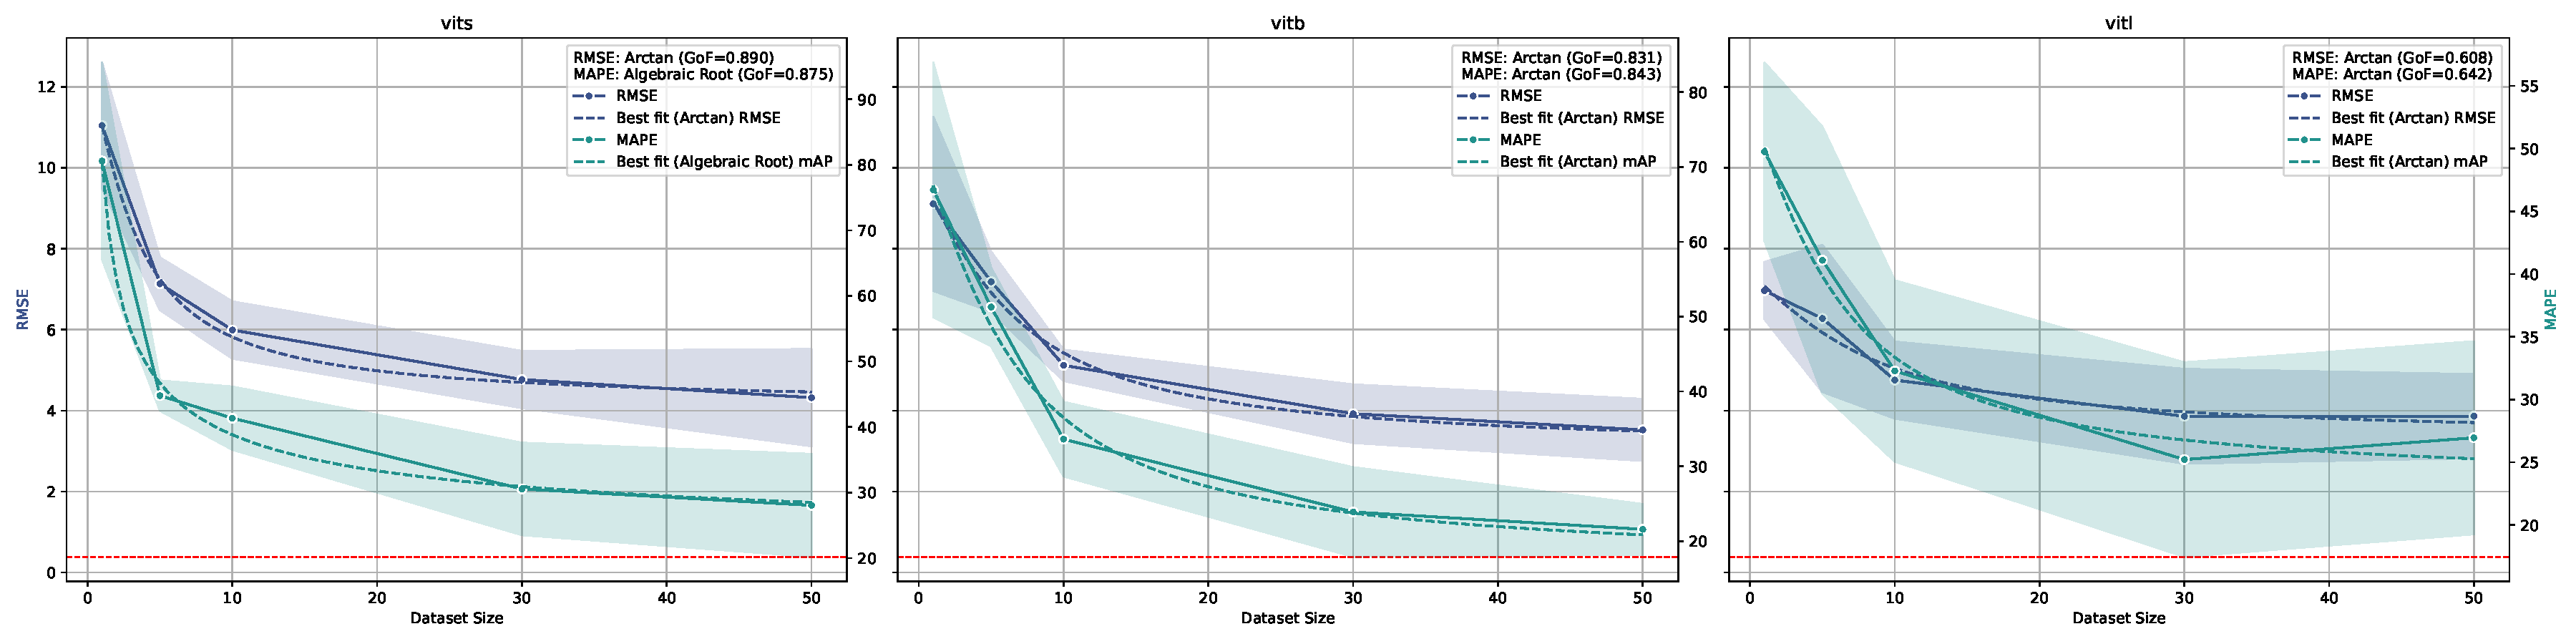
\includegraphics[width=1\linewidth]{Plots/rmse_ap_vs_shots_cdvito.pdf}
  \end{adjustwidth}
  \caption{The figure shows the relationship between shots and model performance
  for the CD-ViTO model trained and tested on ID datasets.
  The x-axis represents the number of shots.
  The solid lines represent the mean values, while the dashed lines indicate the shots amount/metric 
  prediction model. The left and right y-axis represents the $RMSE$ and MAPE values respectively.
  The red dashed horizontal line represents the benchmark $RMSE$ value of 0.39. The combined
  legend in the upper right corner of each subplot shows the goodness of fit ($GoF$) for both $RMSE$
  and MAPE.}
  \label{fig:shots_vs_performance2}
\end{figure}
\end{landscape}
\clearpage
}

The best result achieved by the CD-ViTO model was a $RMSE$ of 3.9 with ViT-B backbone and 
50 shots to build the prototypes, which is substantially worse than the benchmark value of 0.39 (10 times higher). 
This corresponds to a MAPE on counting of about 25% 
and a $mAP$ of about 0.5 (Figures~\ref{fig:shots_vs_performance1} and \ref{fig:shots_vs_performance2}).
It corresponds roughly to a miscounted plant over four as it is visible looking to
some predictions of this model in Figure~\ref{fig:annotations_few-shots}.
The models fitted on metrics show a reliable $GoF$ for all
the metrics, indicating that the model performance is highly predictable by the number of shots.
These also show that any CD-ViTO size model would not achieve the
benchmark with any shot amount, even if the number of shots were increased beyond those tested.

\afterpage{%
\clearpage
\begin{landscape}
\begin{figure}[p]
  \centering
  \begin{adjustwidth}{-5cm}{-0cm}
  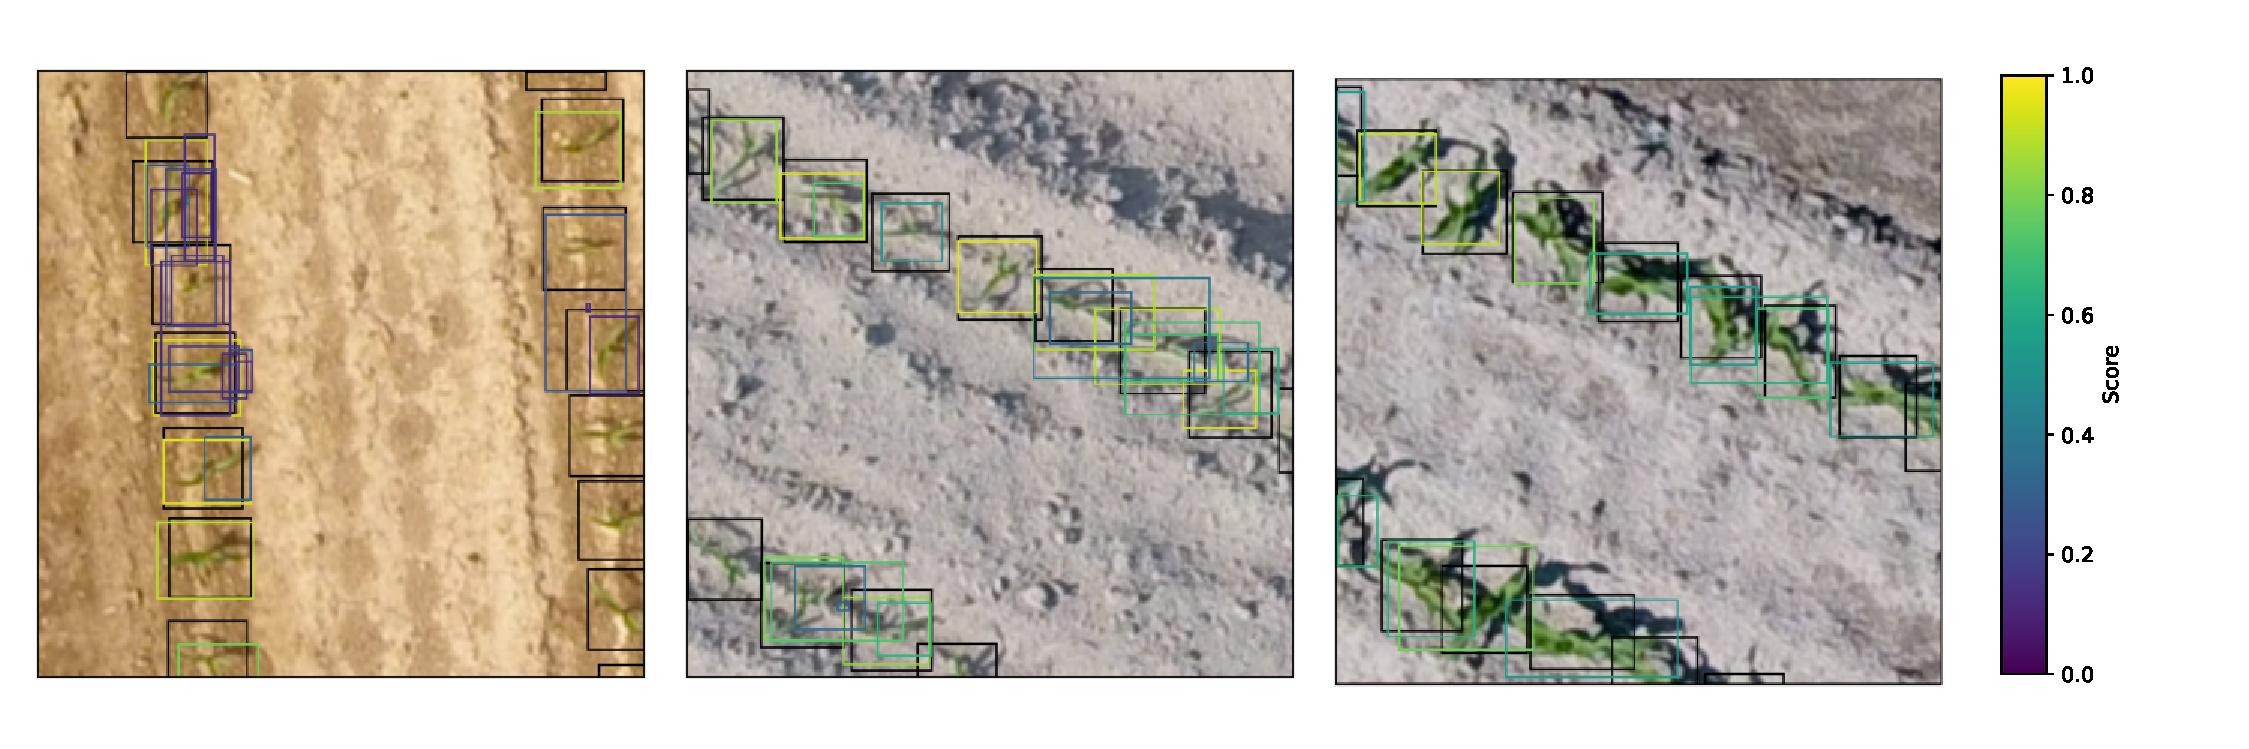
\includegraphics[width=1\linewidth]{Plots/few_shot_annotations.pdf}
  \end{adjustwidth}
  \caption{50 shots CD-ViTO with ViT-B backbone predictions on the 
  1, 2 and 3 ID test datasets tile examples, respectively from the left hand side to the right.
   Black bounding boxes are the ground truth annotations, while the bounding boxes 
   in viridis color scale are the model predictions.}
  \label{fig:annotations_few-shots}
\end{figure}
\end{landscape}
\clearpage
}

\subsection{Zero-shots object detectors}

Figure \ref{fig:zeroshots_vs_performance} shows the relationship between the zero-shots 
model settings and model performance tested on ID testing datasets. Not all the 
model settings were able to predict the whole testing dataset. For example, the 
owlv2-base-patch16-finetuned model was not able to generate any prediction with 
any prompt for any image of the ID testing. A dataset size relationship with metrics 
could not be established as zero-shots models do not require fine-tuning training 
data.
None of the zero-shots model settings reached the benchmark. This is particularly true for the 
$R^2$ values, which were always below 0, indicating poor predictive performance. The 
$RMSE$ values ranged from approximately 5 to 25, significantly higher than those 
observed in the many-shots and few-shots models. Additionally, MAPE values were 
also considerably elevated, ranging from around 40 to 140. Furthermore, the 
$mAP$ values were lower than those of the many and few-shots models for all model 
settings, except for the owlv2-large-patch14-finetuned model, for which very few 
images were successfully predicted with an 
$mAP$ comparable to that of the best few-shots model (50-shots ViT-B backbone).
Some rare case of good predictions were even more accurate than the few-shots best performance, 
as shown in Figure \ref{fig:annotations_zero-shots}.

\afterpage{%
\clearpage
\begin{landscape}
\begin{figure}[p]
  \centering
  \begin{adjustwidth}{-5cm}{-0cm}
  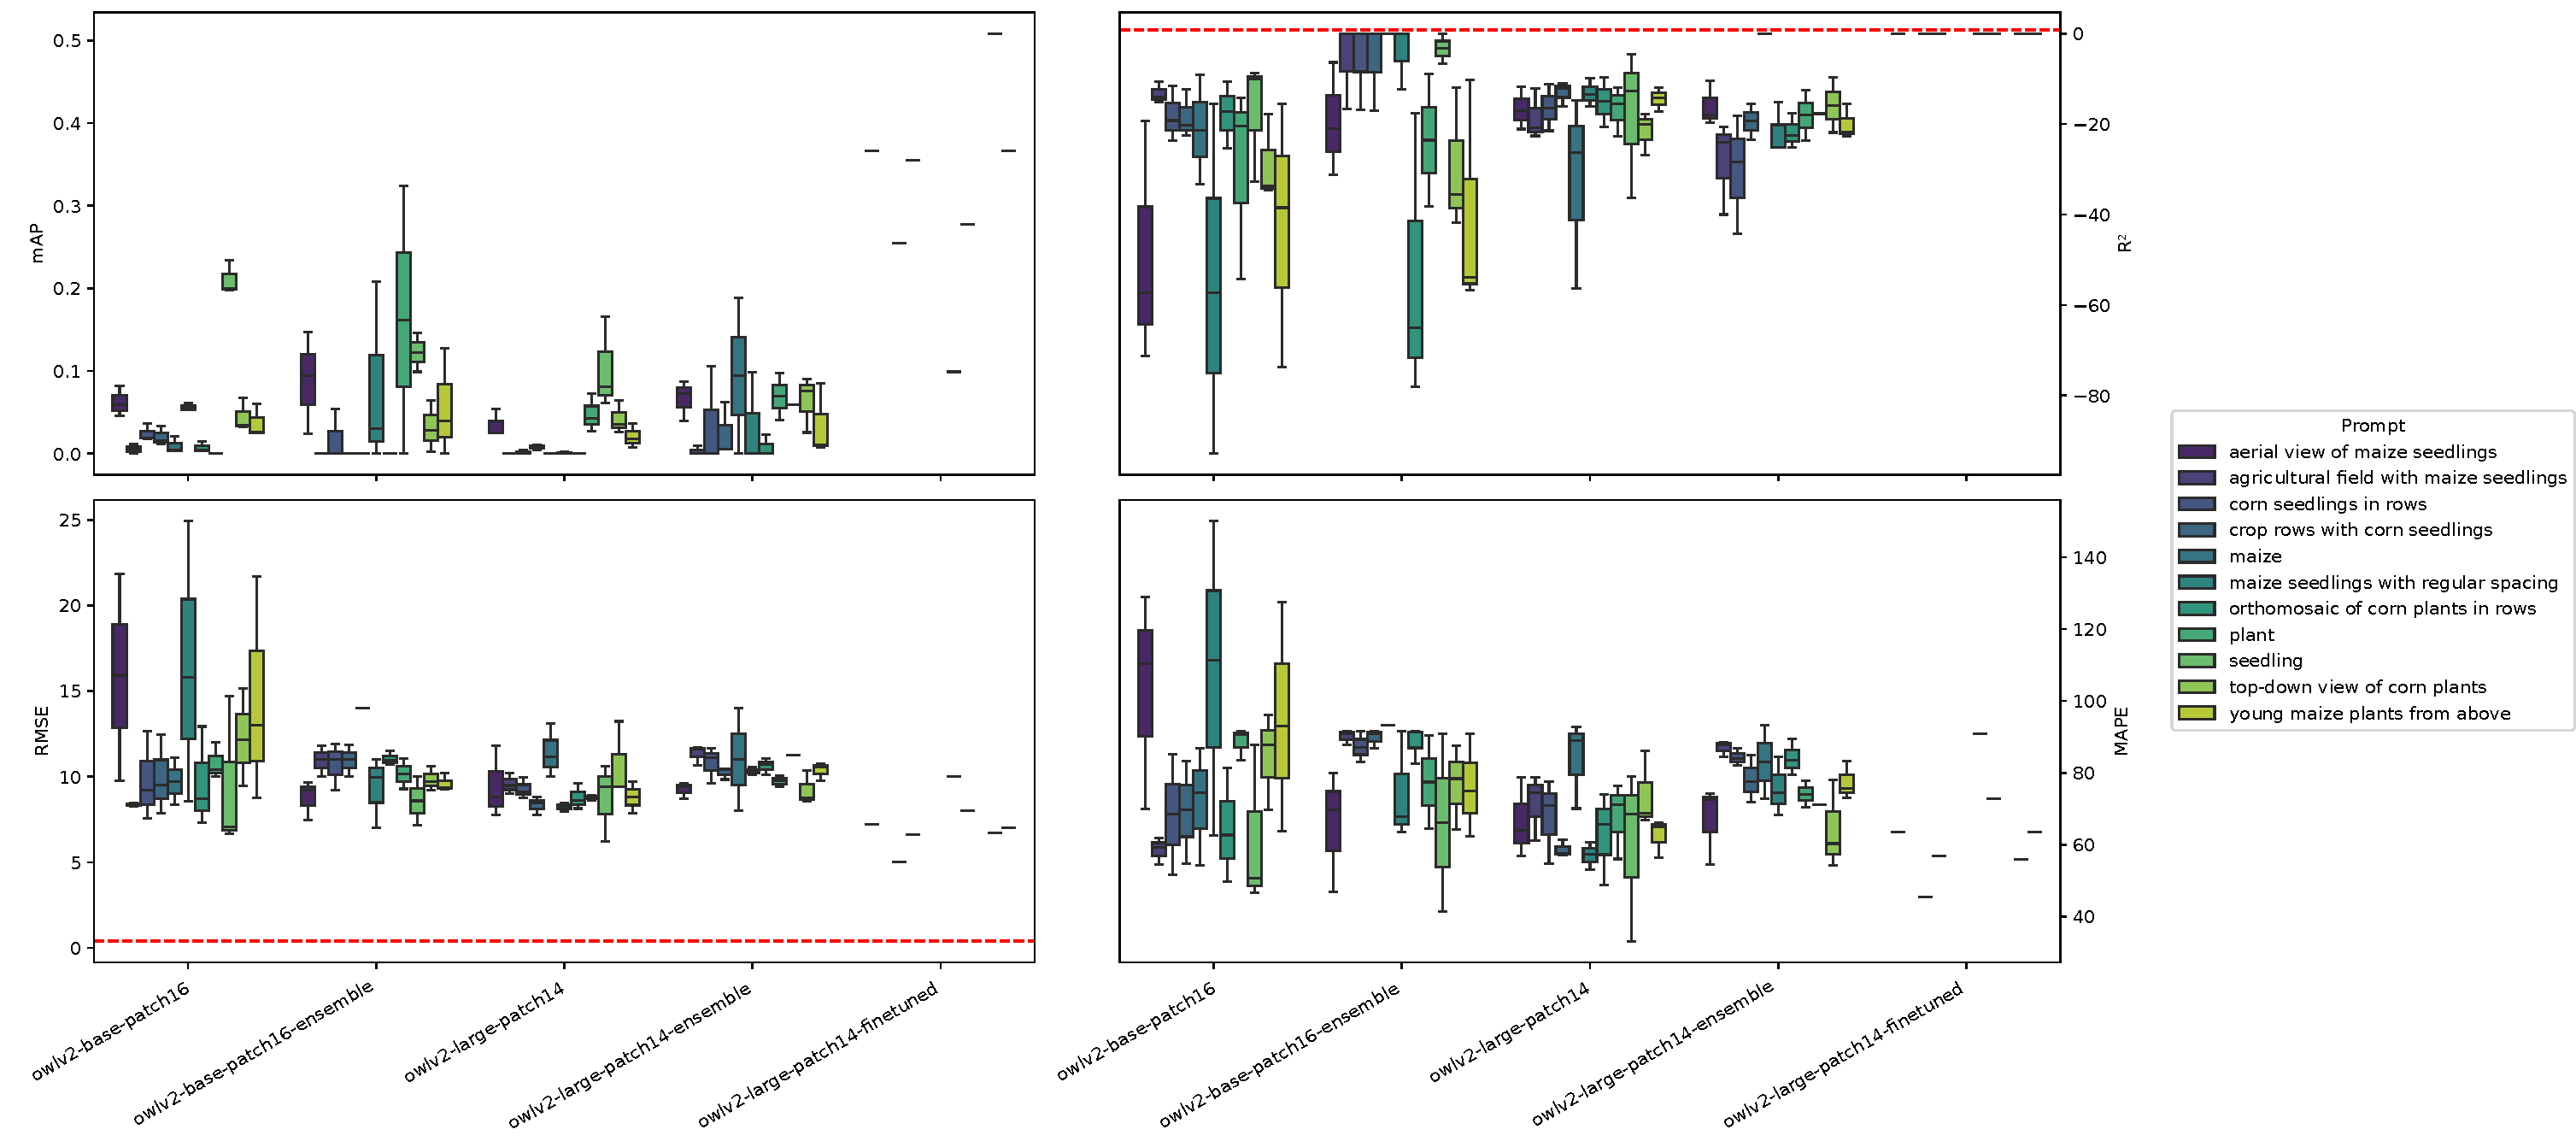
\includegraphics[width=1\linewidth]{Plots/zeroshot.pdf}
  \end{adjustwidth}
  \caption{The figure shows the relationship between the OWLv2 model size, used prompt 
  and model performance.
  The x-axis represents the model settings and the model size.
  Colors represent the different prompts used.
  The four subplots show the $mAP$ (upper left corner), $R^2$ (upper right corner),
  $RMSE$ (lower left corner), and MAPE (lower right corner) values.
  The red dashed horizontal line in the $R^2$ and the $RMSE$ subplots represents 
  respectively the benchmark of 0.85 and 0.39. }
  \label{fig:zeroshots_vs_performance}
\end{figure}
\end{landscape}
\clearpage
}

\afterpage{%
\clearpage
\begin{landscape}
\begin{figure}[p]
  \centering
  \begin{adjustwidth}{-5cm}{-0cm}
  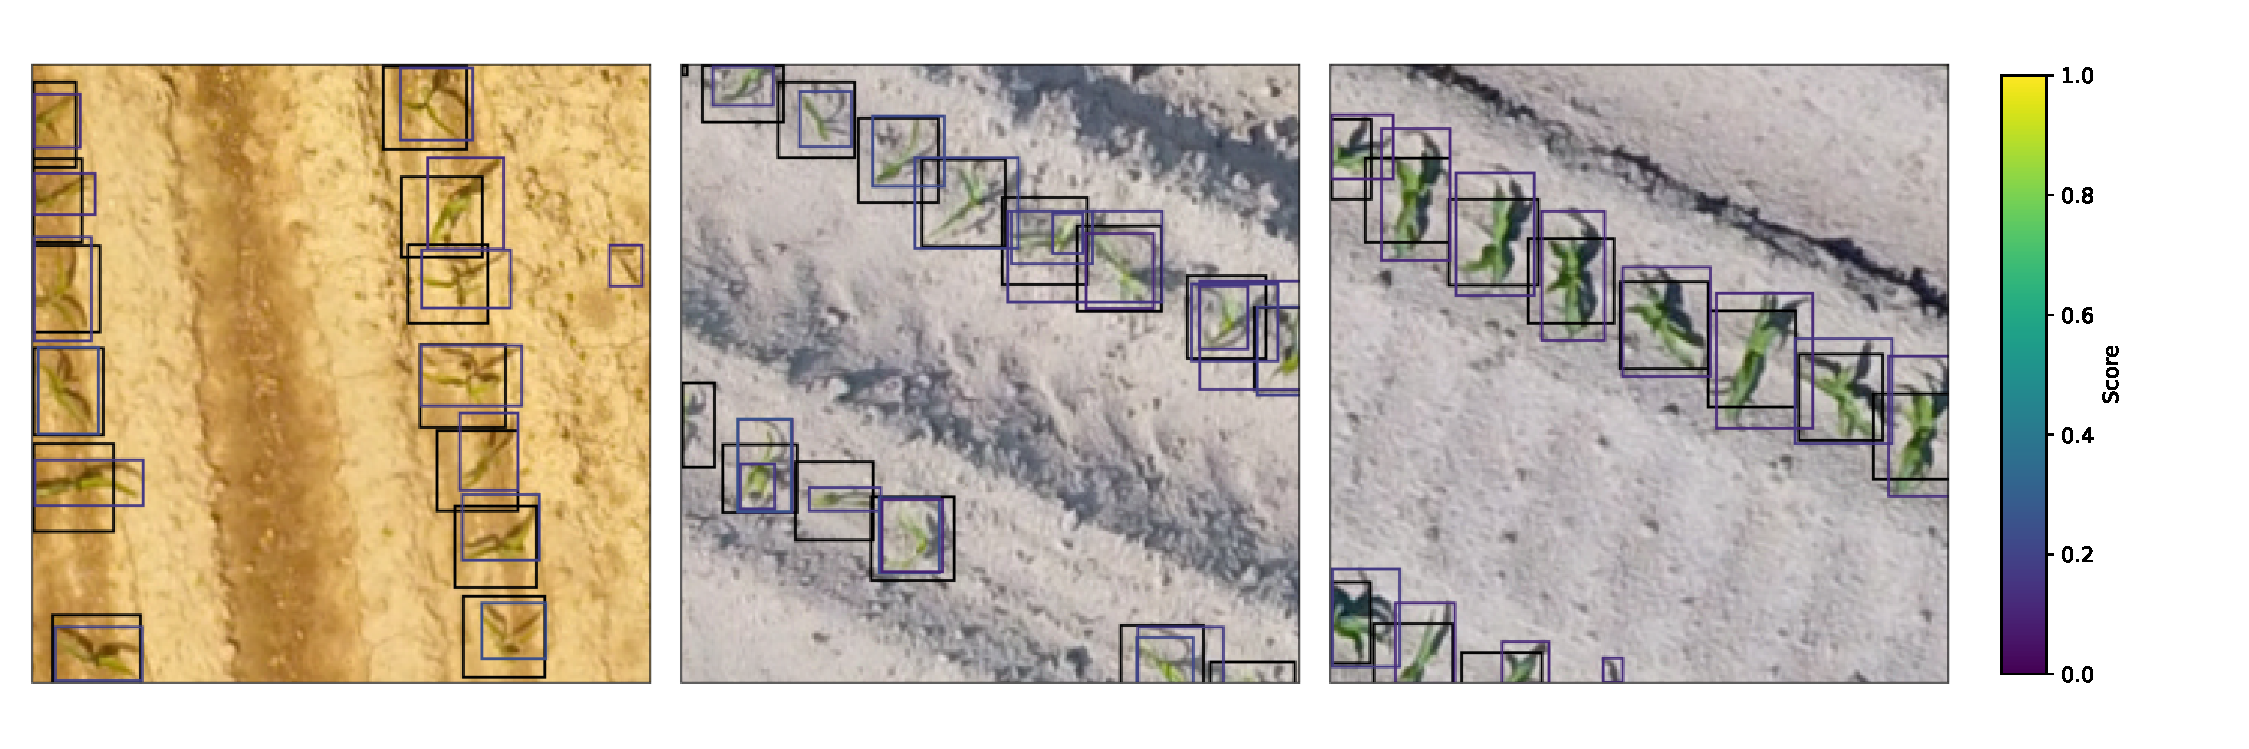
\includegraphics[width=1\linewidth]{Plots/zeroshot_images.pdf}
  \end{adjustwidth}
  \caption{The best predictions with the OWLv2 model.  
  The ID\_1, ID\_2 and ID\_3 datasets respectively from the left hand side to the right.
  Prediction with owlv2-base-patch16-ensemble model of the ID\_1 dataset,
  and with owlv2-base-patch16 model on the other two datasets.
  All the predictions are made with the prompt "seedling".
  Black bounding boxes are the ground truth annotations, while the bounding boxes 
  in viridis color scale are the model predictions.}
  \label{fig:annotations_zero-shots}
\end{figure}
\end{landscape}
\clearpage
}


%%%%%%%%%%%%%%%%%%%%%%%%%%%%%%%%%%%%%%%%%%
\section{Discussion}

\subsection{Dataset Source Impact on Object Detection Performance}
Our experiments clearly demonstrate the critical importance of dataset source 
for successful arable crop seedling detection. None of the tested models, regardless 
of architecture or parameter amount, achieved the benchmark $R^2$ value of 0.85 
when trained on out-of-distribution (OOD) datasets. 
Several inherent biases in our datasets likely influenced model performance.
This aligns with previous findings 
by David et al. \cite{davidPlantDetectionCounting2021}  and Andvaag et al. \cite{andvaagCountingCanolaGeneralizable2024}, 
who similarly reported significantly 
lower performance when using training samples from sources different from the inference dataset.

The domain gap challenge is particularly pronounced in agricultural applications, 
where environmental conditions, lighting, camera parameters, and plant growth stages 
vary substantially across datasets. The failure of OOD training highlights that visual 
features learned from one orthomosaic do not generalize well to others without 
significant adaptation. 
As the goodness-of-fit ($GoF$) of the models explicating the relationship between dataset size and performance
was always below 0.2, one can argue that the interval of dataset size tested was too narrow
to achieve a good fit or that other variables play an important role in determining model performance.
Both cases are likely to be true, but also the maximum OOD dataset size that
was tested (1168) was really small in respect to other studies that use training 
datasets of tens of thousand of images to achieve such benchmarks \cite{badgujarAgriculturalObjectDetection2024}.
This further highlights the importance of collecting in-domain training data, 
as the minimum OOD dataset size and quality to train an object detector to
count arable crops seedling that generalizes to all the real-world cases
is difficult even to establish with a limited dataset. 

Despite the poor performance of OOD dataset trained models, some of them showed a low $MAPE$ value of less than 20\%,
not enough to consider the models for direct inferencing but rather as an annotation
tool for the ID dataset.

\subsection{Many-Shot Object Detection: Architecture and Dataset Requirements}
Our results reveal important relationships between model architecture, count metrics, 
and minimum dataset requirements. Within YOLO-family models, we observed that the lightweight 
YOLOv5n, YOLOv5s, and YOLOv8n achieved the benchmark with 130, 130, and 110 samples respectively. 
As already well-known, increasing model complexity in CNN-based architectures corresponded to increased 
dataset size requirements.
Conversely, for transformer-mixed models like RT-DETR, we observed different patterns, with RT-DETR L achieving 
the benchmark with only 60 samples while the larger RT-DETR X required 100 samples. The
empirical models of dataset size versus performance showed comparable $GoF$ between RT-DETR and YOLO-family models,
except for YOLOv5n which showed a particularly high $GoF$. This suggests that transformer-based models have
the same predictability to reach the benchmark with the reported dataset size as the CNN-based models, except
for YOLOv5n which has a higher predictability to reach the benchmark given the same dataset size.
Overall, transformer-based models may require fewer samples to achieve the same performance as CNN-based models,
potentially due to their ability to capture long-range dependencies and contextual information more effectively.
A visible side-effect of the adoption of transformer-mixed models is the higher computational cost
of the training phase in terms of time and memory, that could be a limitation for some applications.
This creates a practical tradeoff for practitioners: whether to use a simpler CNN-based model like YOLOv5n 
and invest in collecting more annotated images (approximately 130), or to allocate more computational 
resources for a transformer-mixed model like RT-DETR L that can achieve comparable performance with 
roughly half the amount of labeled data (approximately 60 images).

The predictability of model performance based on dataset size (as evidenced by $GoF$ values exceeding 0.3 
for successful models) provides practical guidance for practitioners. The relationship between dataset 
size and performance (modeled using logarithmic, arctangent, or algebraic root 
functions, depending on best fit) suggests diminishing returns beyond certain thresholds, 
which can help inform efficient resource allocation for annotation efforts.

\subsection{Dataset Quality Trade-offs}
Our investigation into minimum dataset quality requirements revealed that models can tolerate some reduction 
in annotation quality while still maintaining benchmark performance achieved with the
same training dataset size. YOLOv5n, YOLOv5s, and YOLOv8n achieved 
the benchmark with 85\%, 90\%, and 85\% of the original dataset quality, while RT-DETR X required 
only 65\%. Notably, RT-DETR L failed to maintain benchmark performance with any reduction in annotation quality, 
suggesting different sensitivity to annotation errors.

This difference in quality tolerance between RT-DETR L and RT-DETR X can be explained by considering their 
respective minimum dataset sizes. RT-DETR L was tested with quality reductions on its minimum benchmark-achieving 
dataset size of just 60 samples, while RT-DETR X was tested with 100 samples. With fewer training examples, 
RT-DETR L becomes more sensitive to the quality of each individual annotation, as each annotation represents 
a larger proportion of the total learning signal. In contrast, RT-DETR X, with its larger training dataset, 
can better compensate for quality reductions by leveraging redundancy across more examples.

These findings provide valuable insights for practical applications, as they suggest that in some 
cases, it may be more efficient to collect a larger quantity of moderately-quality annotations 
rather than focusing on perfect annotations for a smaller dataset. This also indicates potential 
for semi-automated annotation workflows, where machine assistance in annotation (which may introduce 
some errors) could be acceptable for many applications.

\subsection{Few-Shot and Zero-Shot Approaches: Current Limitations}
Despite recent advances in few-shot and zero-shot learning, our experiments reveal significant 
limitations in these approaches for precise maize seedling detection. The best CD-ViTO few-shot 
model achieved a $RMSE$ of 3.9 with 50 shots (using ViT-B backbone), substantially below the benchmark 
requirement of 0.39. Similarly, zero-shot models like OWLv2 performed poorly regardless of prompt 
engineering efforts.

These results contrast with the promising performance reported for few-shot and zero-shot methods 
in general object detection benchmarks \cite{xuDeViTDecomposingVision2023,mindererScalingOpenVocabularyObject2023}. 
Several factors may explain this gap: 
First, the domain-specific nature of aerial maize seedling imagery, where subtle 
textural differences and high intra-class variability are prevalent, severely challenges 
models pre-trained on general object detection datasets. As illustrated in the few-shot 
experiments (Figure \ref{fig:shots_vs_performance1}), increasing 
the number of shots leads to nonlinear improvements in metrics such as R² and $mAP$ 
(following an arctan-like trend), yet the error metric ($RMSE$) remain significantly 
above the benchmark. This saturation effect suggests that even with more than usual maximum tested
prototypes (50 instead of 30), the models struggle to capture the fine-grained visual cues 
necessary for precise seedling detection. Moreover, the zero-shot results (Figure 
\ref{fig:zeroshots_vs_performance}) reveal a pronounced sensitivity to prompt phrasing, with all 
variants, including ensemble and fine-tuned versions of OWLv2, consistently failing 
to approach acceptable error rates. These observations imply that both the inherent 
complexity of the task and the limitations of current few-shot and zero-shot frameworks 
necessitate more domain-specific strategies. Addressing these challenges through 
domain-specific adaptations could help narrow the performance gap, potentially making 
few-shot and zero-shot methods more competitive for arable crop seedling detection.
Interestingly, the few-shot and the zero-shot models were able to detect all the seedlings
without false positives in few cases. It would be interesting to investigate the
possible ways to retain these images and use them to populate the training dataset
for a many-shots model.

\subsection{Handcrafted Methods in the Deep Learning Era}
Despite the focus on deep learning approaches, our handcrafted (HC) object detector 
demonstrated strong performance on the testing datasets ($R^2$ from 0.87 to 0.95). 
However, a significant limitation was the small proportion of tiles (1.8\% to 7.8\%) 
for which it could provide reliable annotations. This illustrates the classic trade-off 
of rule-based systems: high precision in constrained scenarios but limited generalizability.

These findings suggest that HC methods may still have value in a hybrid approach, where 
they provide high-quality annotations on a subset of data, which can then be used to 
bootstrap deep learning models. Such an approach could be particularly valuable for 
specialized agricultural applications where annotation resources are limited.

This approach is highly adopted in industry, where the HC method is used to
annotate the training dataset and the deep learning model is used to predict the real-world
cases, but it introduces a possible bias in the training dataset that could be a limitation
for the model generalization. The main problem is that the HC1 method relies
on color thresholding that filter the 
objects based on the color of the objects. That could be not the best
way to annotate the training dataset for a deep learning model that could learn
more complex features of the objects, but also the ones selected by the HC1 method.

\subsection{Implications for Practical Applications}
Our study has several practical implications for developing arable crop seedling detection systems.
First, collecting in-domain training data is non-negotiable for achieving benchmark performance. 
Finding a way to automatically obtain the training dataset from the same distribution as the intended 
inference target is a key step in developing a robust object detector for arable crop seedling detection.

The logarithmic relationship between dataset size and performance suggests that initial annotation 
efforts should focus on reaching the minimum viable dataset size (60-130 images depending on architecture), 
after which additional annotations yield diminishing returns. This finding helps organizations optimize 
resource allocation for annotation efforts.

Our results also demonstrate that some reduction in annotation quality is acceptable, with models 
maintaining benchmark performance with 65-90\% of the original quality. This suggests that semi-automated 
annotation workflows could be efficiently implemented for agricultural applications, potentially reducing 
the time and cost associated with manual annotation.

Current few-shot and zero-shot methods, while promising, are not yet viable replacements for traditional 
object detection approaches in seedling detection or counting tasks. However, they might still serve 
auxiliary roles in the annotation pipeline.

Hybrid approaches combining handcrafted methods with deep learning models could provide a practical solution 
for achieving benchmark performance. We observed that OOD many-shots, few-shots, and zero-shots models are 
occasionally able to produce annotations with sufficient quality for training ID many-shots models. A promising 
direction for future work would be to develop methods for automatically identifying and leveraging these 
high-quality annotations. Specifically, the HC2 component of our handcrafted approach could potentially be used 
to filter and validate annotations produced by these models, overcoming the color-thresholding bias introduced 
by HC1 while maintaining the agronomic knowledge encoded in HC2's row-pattern validation.

\subsection{Future Work}
In this study, we focused on the minimum dataset requirements for fine-tuning pre-trained models for the 
downstream task of counting arable crop seedlings through object detection. We did not explore the potential 
benefits of using domain-specific backbones. Future work could investigate whether dataset size requirements 
could be further reduced by using backbones pre-trained on agricultural imagery, particularly aerial 
orthomosaics of crop fields. Such domain-specific pre-training might allow models to learn more relevant 
features for crop detection tasks, potentially reducing the amount of in-domain data needed for fine-tuning.

%%%%%%%%%%%%%%%%%%%%%%%%%%%%%%%%%%%%%%%%%%
\section{Conclusions}

This study demonstrates that successful maize seedling detection requires in-domain 
training data, with out-of-distribution training requiring unreasonable dataset size to 
achieve benchmark performance across all tested models. 
We established minimum dataset requirements for several 
architectures, finding that lightweight YOLO models achieve benchmark performance 
with 110-130 samples, while certain transformer-mixed models like RT-DETR require as 
few as 60 samples. Models showed varying tolerance for reduced annotation quality, 
with some maintaining performance with only 65-90\% of original annotation quality.

Despite advances in machine learning, neither few-shot nor zero-shot approaches currently 
meet precision requirements for arable crop seedling detection. Our handcrafted 
algorithm achieved excellent performance within its constraints, suggesting potential 
value in hybrid approaches combining rule-based methods with deep learning. These 
findings provide practical guidance for developing maize seedling detection 
systems, and possible ways to overcome the limitations of the current deep learning
models for this application.

\bibliographystyle{plainnat}
\bibliography{Phd_Thesis_SBumbaca}

\end{document}